\chapter[Password Personality]{Understanding Password Practices through the Lens of Personality Traits}\label{chap:pws_and_personality}

%\section{Introduction}
% general introduction
% show that not *everyone* does the same
% selection is an individual task, not everyone selects passwords in the same way
Although there are certain general patterns, password selection is a task that each individual handles in their own way. 
% even perception differs.
We have shown in Chapter \ref{chap:pasdjo} that password strength is \textit{subjectively evaluated} depending on certain characteristics whose benefits users interpret in different ways. Again, while there was an overall tendency, we were unable to break down the strength ratings by such individual differences: was there a special user group who performed better than others in the game? What characterizes this user group? Moreover, our previous chapter shed light on password policies in the wild. In a few notable cases, the rules were challenging and reject a substantial part of passwords. Users have developed strategies to cope with rejected passwords, but it would be interesting to know the exact factors that contribute to their behavior in these circumstances. Egelman and Peer make a strong argument that there is no ``average user'' so it is necessary to look at individual differences to understand user behavior \cite{Egelman2015AverageUser}. 

% personality traits in cybersecurity are a thing
Demographic background is one of the external factors that influences password selection \cite{Mazurek2013Measuring,  Violettas2014PasswordsAvoidGreece, Wang2015ChinesePWs}. Personality traits have been brought into the discussion to explain user preferences, actions, and behaviors in security questions \cite{Brown2004GeneratingPWs, Gross2016EffectCognitiveEffort, Shropshire2006PersonalityITSec, Zakaria2013DesigningEffectiveSecurityMessages}. Especially in research about phishing susceptibility we find evidence that personality traits have the potential to explain behavior \cite{Halevi2013PilotStudyPersonality,Halevi2015SpearPhishing,ParrishJr2009PersonalityPhishing,Uebelacker2014SocialEngineering}. 
% personality traits even matter for passwords
Empirical results from password studies have been discussed and explained with different personality traits, too \cite{Haque2014PsychometricsStrongPassword,Weirich2001PrettyGoodPersuasion}. It is evident that a user's personality shines through when they select a word with personal meaning. 
% characterize personality in this realm
Petrie classified users in distinct password personalities: family-oriented, fans, fantasists, and cryptics\footnote{The original survey is not available online anymore. In a personal inquiry with Ms Petrie, she said that the original data is with the firm who commissioned the survey. The aggregated statistics are available at \url{http://passwordresearch.com/stats/statistic130.html}, \la{29.01.2018}}. A LastPass report more roughly divides password usage into two groups \cite{LastPass2016PersonalitiesGetUsHacked}: Type A users want to stay in control and are driven to act securely, so they developed an elaborate system that they perceive as suitable. Type B users do not believe that their accounts are valuable to attackers, so they do not prioritize security over usability. 
% this kind of categorization is nice, but too rough, maybe something more sound would solve the situation.
Those two taxonomies stem from analysis of user-selected passwords, i.e. a retrospective evaluation. However, predictive approaches are under-explored. For instance, if a user is generally an emotional person, does this impact their password selection strategies? If a user is diligent in real life, do they invest effort to diligently craft passwords, too? 
%``I can't remember passwords anyway'' could be attributed to a person who is less conscientious and/or less neurotic. 
%Are neurotic people more concerned about password strength, because they fear attacks more?

% that's what we do.
In a series of user studies we explored the associations between personality traits and passwords. If such associations exist, they open a new range of support systems that are tailored to a user's personality. Current one-fits-all approaches could be re-designed radically. The research was carried out in cooperation with three students. In each separate project we focused on a different stage of the password life-cycle. Timo Erdelt investigated personality as predictor for the usability of composition policies \cite{Erdelt2017BA}. Paul Huber explored correlations between strength perceptions and personality traits \cite{Huber2016BA}. Finally, Aline Neumann examined personality factors in password selection \cite{Neumann2017BA}. In total, 440 individuals participated in three separate online studies. In the following sections, the projects are put into context and their findings are discussed on a bigger picture. 

\subsubsection*{Research Objectives}
Our primary goal was to find ways to predict password behavior from personality traits. At this point, the discourse about risky passwords included personality factors as hypothetical explanatory variables. However, only few empirical studies had been carried out to challenge the assumptions. We aimed to provide such empirical data and a discussion of the implications on the design of password policies and password authentication systems. For instance, adjusting requirements of password policies depending on the user's personality promises to reduce frustration of password selection. Thus, our over-arching research question can be framed as ``\textit{Does personality influence a user's mental models of password strength and consequently selection and coping strategies?}''.

%more related work: Groß \etal \cite{Gross2016CognitiveDepletion}
%
%Goals/motivation: 
%- some publications tried interpreted their findings as a consequence of different personality traits. first mentioned in \cite{Weirich2001PrettyGoodPersuasion} that personality could make a difference -- however, this had never been tried to empirically measure. 
%- explore differences in certain coping strategies (selection and reuse) through the lens of personality
%- find suitable ways to adjust password policies \cite{Seitz2017PersonalizingPasswordPolicies} - when users need to reset their password, after they had used the service for a while. 
%
%We posed the following research questions before we set out to conduct the study.\\
%\textbf{RQ1 - Psychological Factors} How much do psychological factors affect the perceived strength of passwords?\\
%\textbf{RQ2 - Big-Five vs GDMS} Are the Big-Five traits stronger or weaker predictors for strength perception than other psychological variables?\\
%\textbf{RQ3 - Portfolio Factors} Is the personal password portfolio associated with strength perception?

\section{Background and Related Work}
%We position our work in usable security and privacy, in particular password research. Moreover, we include psychological models to better understand users dealing with passwords. 
In this section we give a brief overview about the characteristics of strong passwords and how users go about creating them. Moreover, we portray projects in usable security and privacy research in which the users' psyche has been the focus. 
% secondary
%premise
%influencing 
%preconditions


%Moreover, since sophisticated attacks often start with checking for already known passwords, obtaining clear text data goes along with attackers improving their approach. A password that was strong before can quickly become very weak.  
%TODO eventuell noch das DING WANG paper und oder das Neural Network Ding vom Melicher zitieren.

%\subsection{Studies of Personality in Cyber Security}
\subsection{Sociodemographic and Cognitive Factors}
%TODO subconscious? 
%not exhaustive
% DEMOGRAPHICS
Apart from such conscious behavior, there may be other preconditions that make some users pick stronger passwords than others. In a large field study, Mazurek et al. found that computer science and engineering students created passwords that were less guessable than those from business or politics students \cite{Mazurek2013Measuring}. Beyond demographic background, context factors like the emotional state during password selection have also been investigated. 
% EMOTIONS
Gulenko examined the effect of presenting positive textual messages and icons during password selection and found benefits for the adoption of passphrases \cite{Gulenko2014PasswordsEmotion}. In contrast, putting users in a state of cognitive distress or depletion made participants choose weaker passwords in a large lab study \cite{Gross2016EffectCognitiveEffort}. 
% PAST EXPERIENCES / BREACHES / ATTACKS
Social pressure as another type of psychological leverage was investigated by Egelman \etal \cite{Egelman2013DoesMyPasswordGoUpToEleven}. While they argue that account value plays a superior role for the effectiveness of password meters, others have shown that the \textit{design} of a password meter does have a measurable impact on the effort users put into creating a password \cite{Ur2012HowDoesYourPasswordMeasureUp}. In summary, the literature shows that password selection depends on context factors beyond education and experience. 


\subsection{Personality Factors in Cyber Security}
In our work, we are interested in context factors of password strength originating from psychological variables like personality. One of the most commonly used models to characterize personality are the Big-Five traits (B5), also known as the five-factor model. Costa and McCrae \cite{Costa1992NEO} refer to the personality traits as \textit{openness to experience}, \textit{conscientiousness}, \textit{extraversion}, \textit{agreeableness}, and \textit{neuroticism} (OCEAN). The traits can be described with these exemplary adjectives \cite{McCrae1987ValidationFFM}:\\
\textbf{Openness:} imaginative, creative, curious, independent, liberal\\
\textbf{Conscientiousness:} careful, reliable, ambitious, scrupulous, neat, punctual\\
\textbf{Extraversion:} sociable, talkative, passionate, warm\\
\textbf{Agreeableness:} selfless, helpful, forgiving, cheerful, humble\\
\textbf{Neuroticism:} worrying, emotional, insecure, impatient, vulnerable, subjective

Most frequently, the influence of these personality traits have been explored for privacy-concerns, where the openness trait was associated with privacy attitudes \cite{Egelman2015PredictingAttitudes,Minkus2014PersonalizationPrivacy}. Other inquiries have shown that personality traits like neuroticism \cite{Halevi2013PilotStudyPersonality} or openness \cite{Uebelacker2014SocialEngineering} might be associated with the response to phishing attacks. The likelihood of employees adhering to security policies is potentially influenced by the manifestation of agreeableness and conscientiousness \cite{Shropshire2006PersonalityITSec,Shropshire2015}. These investigations show that personality  models are a considerable factor in security and privacy. Yet, our understanding of the influence of personality on password perception and consequently password selection is still low. Our work tries to improve our understanding about the origin of the differences in users' judgments of password strength. 
%is linked to these aspects, because passwords protect privacy of users and sensitive data of companies. %However, how password behaviors are formed and how much of the  is explained by psychological factors is still underexplored
%Malkin2017PersoanlizedSecurityMessaging

%%%%%%%%%%%%%%%%%%%%%%%%%%%%%%%%%%%%%%%%%%%
%%%%
%%%%
%%%%			STUDY  1 ONE EINS
%%%%			POLICIES
%%%%
%%%%
%%%%%%%%%%%%%%%%%%%%%%%%%%%%%%%%%%%%%%%%%%%
\section{Study 1: Policies}\label{sec:personality:study-1}
% general motivation - why do we investigate this?
We start out with the exploration of psychological factors for the design of password policies. We were motivated by the fact that, at this point, policies are a one-fits-all solution that evidently does not work in the same ways for all users: Shay \etal observed that subjective usability ratings for policies differed among participants \cite{Shay2012CorrectHorseBatteryStaple, Shay2014CanLongPasswordsBeSecureAndUsable}. For instance, about 40\% of their participants found it difficult to create a password under a ``3class16'' policy, but another 40\% found it easy \cite{Shay2014CanLongPasswordsBeSecureAndUsable}. Following the general discourse and related results from privacy research, we hypothesized that an individual's personality might be responsible for their attitudes towards one policy or another. Therefore, our goal in this project was to explore such associations between personality traits and policy preference. At this point, we leave out analyses on password strength.
%GOALS: explore associations between big-five traits and password selection under different policies, both on usability and security metrics. Investigate the effects of using a non-traditional password policy based on emojis. user preference for one policy or another. explorative study so no p-values.
\subsection{Method}
% general methodology
Our study was completely exploratory, because the literature did not allow us to derive narrow hypotheses. Since personality traits are nuanced, we opted for an online survey to collect a large sample. Personality was assessed based on the Five-Factor Model. We opted for the very reliable BFI-K construct by Rammstedt and John \cite{Rammstedt2005BFI}, which is also freely available in German. Moreover, with its 21 items, the time to fill out the questionnaire is kept reasonably low. 
Participants were asked to create several passwords in a row, i.e. the study followed a within-groups protocol. Here, we evaluated three different password policies: a traditional (3class12), an uncommon (2word12), and a novel policy (emoji12) that required the selection of at least one emoji through a graphical user interface (more on emojis in Chapter \ref{chap:emojipasswords}). The reason for this choice was that the policies are different enough to serve as characteristic levels of the independent variable ``policy''. Also, creating passwords that exceed the length requirements of typical policies (see Chapter \ref{chap:policies_reuse}) is more difficult, so we could better measure the differences of perceived difficulty. Participants assessed the ``difficulty to create'' of a password for each policy. Moreover, we had them rank the policies by their personal preference, so the distinctiveness of 3class12, 2word12, and emoji12 would help them spot and judge the differences easily, which makes the data more reliable.

\subsubsection{Structure and Tasks}
The study was divided into 3 overall parts. In the first part, participants were briefed about privacy details of the study and they provided demographic background information. Then they proceeded to the personality questionnaire before they were asked to perform three experimental tasks. Each consisted of creating a password and assessing the difficulty with agreement levels on the three items \textit{``It was difficult to create a password that meets the requirements''}, \textit{``I found the password requirements bothersome''}, and \textit{``It was easy to create a \textit{new} password''}. Agreement was measured on a five-point scale ranging from ``Strongly disagree'' to ``Strongly agree''. Inversely keying the items as well double encoding makes the data more robust against implausible responses. The resulting difficulty-to-create score thus ranges from 3 to 15 (3 = very easy, 15 = very difficult).

The order of the policies was counterbalanced during the experiment to mitigate order effects. For each participant, we recorded the resulting order as a control variable. We chose an online-banking scenario for all three selection tasks. The first prompt was to create a password to protect an online banking account. Secondly, participants were told that someone had gained access to their account and the bank locked them out. As a security precaution, they had to reset their first password. The last task description explained that their password had expired after one year and they need to reset it again. This storyline was designed to fulfill the \textit{realistic threat} principle proposed by Krol \etal (see Section \ref{sec:rw:principles-experiments}) \cite{Krol2016ExperimentDesign}. 

We used SosciSurvey, a standard survey tool, to collect the responses. The dynamic parts involving password selection were embedded in iframes. To match the data from the survey tool and the iframe we used URL query parameters containing the response ID. We asked participants to only use a desktop browser to avoid styling glitches and unexpected behavior from the prototypes. %Auto-complete was prevented in any case

\subsubsection{Recruiting and Demographic Background}
We recruited participants through posts on social networks and by sending out the invitation link in a university-wide newsletter (more than 5000 recipients), which was due to time and budget constraints. To incentivize participation, we announced a raffle of five shopping vouchers with a value of 20€ each. At this point, 222 people had started participation. After drop-out and plausibility checks, the remaining sample size was $N=164$. As expected, the age distribution was narrow: our sample consisted mostly of students in their mid-twenties (average age 24 (SD=5). 79 respondents were female, 83 male, and 2 preferred not to answer. In the background screener, 65 people (40\%) indicated to possess formal training in computer science or information technology. We also requested self-reported assessments on password practices. Here we found that 40\% reuse passwords without modification, 32\% reuse them with modifications or with a mnemnoic technique. 17\% often create new passwords. In terms of management strategy, the majority (53\%) tries to memorize passwords. 11\% use a password manager or generator. Written cues served as aid for 10\% of respondents, and 16\% write passwords down on analog media, while 21\% use electronic files. %Interestingly, the distribution of coping strategies is very close to survey findings gathered with more diverse samples \cite{CSID2012PasswordHabits}. Hence, we believe to have caught a representative snapshot of password practices.

\subsubsection{Statistical Analyses}
For statistical analyses, we consulted the StabLab\footurl{http://www.stablab.stat.uni-muenchen.de/}{30.01.2018} to identify suitable methods. After a revision of the collected data and the necessary assumption checks, we analyzed associations by fitting \glspl{GAM} to the dataset. Their advantage over linear regression is that they are more flexible for non-linear associations\footurl{https://en.wikipedia.org/wiki/Additive_model}{30.01.2018}. The \textit{mgcv} package for R was used to calculate the models. GAMs can be primarily interpreted through residual/smooth plots -- the steeper the fitted regression line, the stronger the association (The box in the results section  (\ref{sec:personality:how-to-read-gam}) explains how to read GAM plots in great detail.)

Scores on the Big-Five sub-dimensions served as independent variables, i.e. the predictors in the regression models. \textit{Openness} is coded with five items, while the remaining four dimensions were assessed with four items each. The agreement level for every item was mapped to numeric values from 1 to 5. The score on each sub-dimension is the sum of agreement levels. To better estimate effect sizes, we control for gender, age and IT proficiency in the regression models. 

\subsubsection{Method Limitations}
The method, albeit carefully executed, faces a few limitations regarding the interpretability of the data. First, the sample was fairly homogeneous, because participants were mostly between 20 and 28 years old and have an academic background. This might reduce statistical power in detecting effects on personality \cite{Srivastava2003PersonalityAdulthood}, but on the other hand, this constellation resolves age-related confounding effects. Moreover, our study was strongly focused on individual preferences and usability perceptions of different policies, so only a within-groups design was feasible. However, in real-life password selection, users rarely select three passwords in a row. The choice of our storyline still makes us confident about the ecological validity \cite{Fahl2013EcologicalValidityPasswordStudy}. The repeated measures design did not allow us to measure the policies' influence on password memorability, which we have to postpone to another study. At this stage, the subjective preference was more valuable for our exploration than memorability effects. Besides, we briefed participants to fill out the survey on a desktop PC or a similar device. Since it is always possible to circumvent user-agent detection by requesting the desktop version, we cannot guarantee that all participants followed this instruction, which might have had an effect on their password selection \cite{Melicher2016UsabilityMobileTextPasswords}. 

% we had to redeploy the prototype.
Finally, we unfortunately made a mistake in the deployment of the emoji-based policy. Instead of 12 characters, it required participants to select 16 characters beside the emoji. We realized this fact by looking at descriptive statistics during the course of the study, because the policy performed significantly worse than the other two. We re-deployed the emoji-based policy immediately after we had realized the error. Consequently, we had to remove the data for the creation difficulty and ranking in cases 1-61, reducing the overall sample size to 103. Nonetheless, the sample size is sufficiently large to investigate medium to strong effects. 

%- we started out with emoji16, but made the switch to emoji12 (after 43 participants), because emoji16 received the most negative feedback, but it was mostly due to the length. data removed for ranking (1-61) and difficulty to create (1-43). 

%%%%%%%%%%%
%%%%%%%%%%%
%%%%%%%%%%% Results
%%%%%%%%%%%
\subsection{Results}
Overall, associations between personality and policies were moderate. In the following, we only describe non-trivial and interesting associations. 

\begin{figure}[htbp]
	\centering
	\begin{subfigure}[t]{0.49\linewidth}
		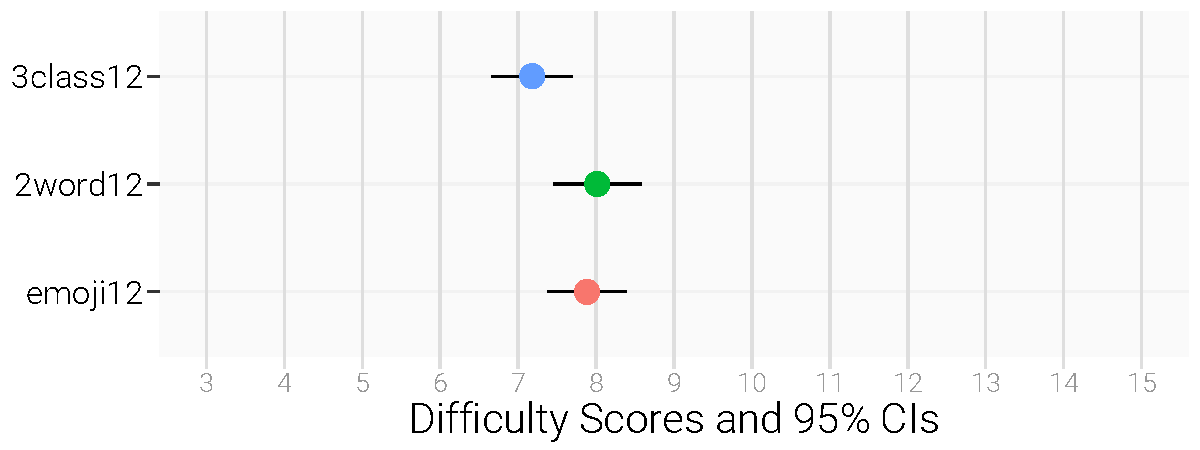
\includegraphics[width=\textwidth]{personality/difficulty-ci}
		\caption{\label{fig:personality:study-1-difficulty-ci}}
	\end{subfigure}
	\begin{subfigure}[t]{0.49\linewidth}
		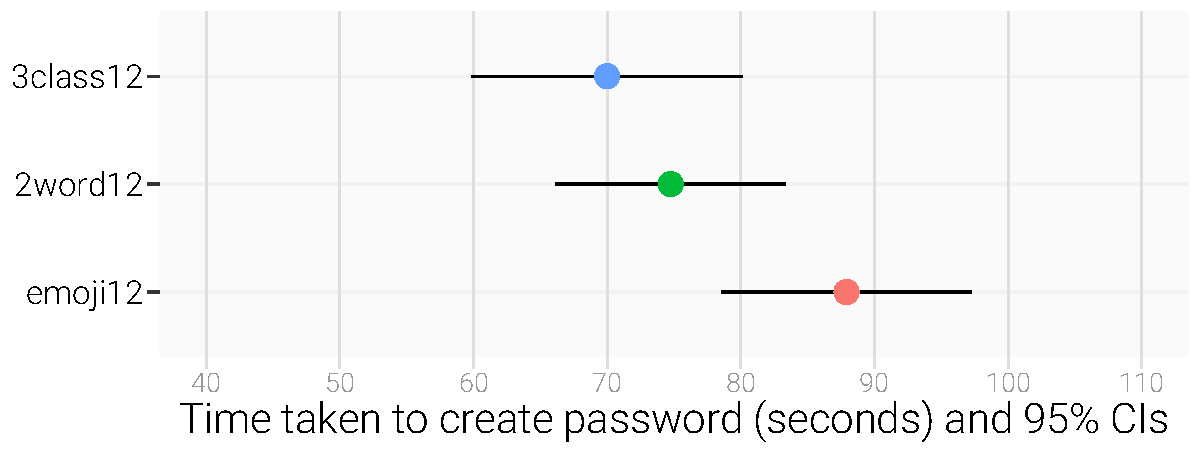
\includegraphics[width=\textwidth]{personality/timing-ci}
		\caption{\label{fig:personality:study-1-timing-ci}}
	\end{subfigure}
	\caption{\label{fig:personality:study-1-usability-stats}Confidence Intervals for a) Difficulty to create and b) time to create passwords in each condition. The traditional policy (3class12) was the easiest and fastest overall, but not on a statistically significant level (also visible in the charts due to the overlapping confidence intervals)}
\end{figure}
\subsubsection{Descriptives and Independent Variables}
Users rated the difficulty to create a password very similarly in all conditions (averages of scores in range [3;15]: 3class12 = 7.18, 2word12 = 8.02, emoji12 = 7.88). A linear mixed model ANOVA did not show significant differences (\statsgt{2+2}{5.28}{0.1}). Figure \ref{fig:personality:study-1-usability-stats} shows the confidence intervals for these two usability metrics ``difficulty to create'' and ``time to create''. Observing no significant differences overall is interesting because it means that individual ratings could be explained by personality traits. %TODO that's not quite clear.



%serial positioning effects do make a difference, but it also appears trivial in the overall sample.
%summary: no big difference between policies and ranking. (this is what makes the remainder more exciting, because a %closer look at the data brings out how the numbers come to be)

%%%%%%%%%%%
%%%%%%%%%%% Difficulty to create a password with a given policy
%%%%%%%%%%%
\subsubsection{Creation Difficulty Models}
The general additive models showed associations between the predictors and creation difficulty scores (see Table \ref{tab:personality:study-1-coffections-clean}). 
\begin{table}[htbp]
  \centering
    \begin{tabular}{l|SS|SS|SS}
          & \multicolumn{2}{c|}{\textit{emoji12}} & \multicolumn{2}{c|}{\textit{2word12}} & \multicolumn{2}{c}{\textit{3class12}} \\ \hline \hline
          (Intercept) & \multicolumn{2}{c|}{$9.99$} & \multicolumn{2}{c|}{$7.04$} & \multicolumn{2}{c}{$6.26$} \\ \hline
\multicolumn{1}{c|}{Predictor}  & \multicolumn{1}{c}{$\beta$} & \multicolumn{1}{c|}{$\sigma_n$} & \multicolumn{1}{c}{$\beta$} & \multicolumn{1}{c|}{$\sigma_n$} & \multicolumn{1}{c}{$\beta$} & \multicolumn{1}{c}{$\sigma_n$}  \\
    Age & 0.02  & 0.06  &       &       & -0.05 & 0.06 \\
    Gender (female) & 0.91  & 0.58  & 1.35  & 0.66  & -0.46 & 0.61 \\
    No IT Background & -0.10 & 0.59  & 0.60  & 0.66  & 0.21  & 0.63 \\
    Extraversion & -0.05 & 0.08  &       &       & -0.01 & 0.08 \\
    Conscientiounsness & 0.01  & 0.09  &       &       & 0.08  & 0.10 \\
    Neuroticism & -0.22 & 0.09  &       &       & 0.05  & 0.09 \\
    \textit{emoji12} Position 2 & 0.52  & 0.65  &       &       &       &  \\
    \textit{emoji12} Position 3 & 0.23  & 0.63  &       &       &       &  \\
    \textit{2word12} Position 2 &       &       & -0.38 & 0.74  &       &  \\
    \textit{2word12} Position 3 &       &       & -0.07 & 0.73  &       &  \\
    \textit{3class12} Position 2 &       &       &       &       & 1.19  & 0.66 \\
    \textit{3class12} Position 3 &       &       &       &       & 0.77  & 0.69 \\ \hline
%    edf: s(Age) & \multicolumn{2}{c|}{} & \multicolumn{2}{c|}{1.81} & \multicolumn{2}{c}{} \\
%    edf: s(Agreeableness) & \multicolumn{2}{c|}{3.27} & \multicolumn{2}{c|}{2.77} & \multicolumn{2}{c}{2.02} \\
%    edf: s(Openess) & \multicolumn{2}{c|}{2.50} & \multicolumn{2}{c|}{1.79} & \multicolumn{2}{c}{1.53} \\
%    edf: s(Extraversion) & \multicolumn{2}{c|}{} & \multicolumn{2}{c|}{1.52} & \multicolumn{2}{c}{} \\
%    edf: s(Conscientiousness) & \multicolumn{2}{c|}{} & \multicolumn{2}{c|}{3.32} & \multicolumn{2}{c}{} \\
%    edf: s(Neuroticism) & \multicolumn{2}{c|}{} & \multicolumn{2}{c|}{1.53} & \multicolumn{2}{c}{} \\ \hline
    Explained Deviance & \multicolumn{2}{c|}{0.15} & \multicolumn{2}{c|}{0.21} & \multicolumn{2}{c}{0.10} \\
    Num. Observations. & \multicolumn{2}{c|}{119} & \multicolumn{2}{c|}{119} & \multicolumn{2}{c}{119} \\
    Num. Smooth terms & \multicolumn{2}{c|}{2} & \multicolumn{2}{c|}{6} & \multicolumn{2}{c}{2} \\\hline
    \multicolumn{7}{l}{\textit{Description:}} \\ 
    \multicolumn{7}{l}{$\beta$ = Correlation coefficient} \\
    \multicolumn{7}{l}{$\sigma_n$ = standard error} \\
    \multicolumn{7}{l}{edf = estimated degrees of freedom by non-linear effects} \\
    \multicolumn{7}{l}{(\glqq estimated degrees of freedom\grqq)} \\
    \multicolumn{7}{l}{Smooth terms = non-linear effects in the model} \\
    \end{tabular}%
  \caption{Additive regression models for the difficulty to create passwords under the three policies.}
\label{tab:personality:study-1-coffections-clean}
\end{table}%
\paragraph{Control Variables} 
The GAM allowed us to model associations linearly for the control variables (example for emoj12 in Figure \ref{fig:personality:dc-emoji-b5}). Although we have to be careful not to generalize too strongly with our sample, linear associations at least enable us to use correlation coefficients $B$ as basis for discussion.
% gender
Female participants assessed it slightly more difficult to create passwords under the emoji12 ($B=0.91$) and 2word12 ($B=1.35, p<0.05$) policies than male participants. For 3class12, the correlation was smaller ($B=-0.46$) and pointed in the opposite direction. 
% it background
Having a background in IT positively showed medium correlations with difficulty in the 2word12 policy, too ($B=0.61$). This policy, albeit alphanumeric, is uncommon in the wild and ignores the verdict of high complexity -- IT people might be skeptical about the ``words'' requirement, while others are less concerned about it.
% order of the policy
The task order also showed medium-strong influence on creation difficulty. If emoji12 or 3class12 were part of the second task, creation was seen as more difficult ($B_{emoij12-pos2}=0.52$),  ($B_{3class12-pos2}=1.19$). 
% age
% we observed non-linear associations between age and creation difficulty, but the small age range forbids us to make conclusive inferences from our data.

%, too: emoji12 ($B=-0.10$) trivial, 3class12 ($B=0.21$) weak, 2word12  medium. it looks as though people with higher IT knowledge struggle with a word-based policy, potentially because it is much less common in the wild. 

\begin{figure}
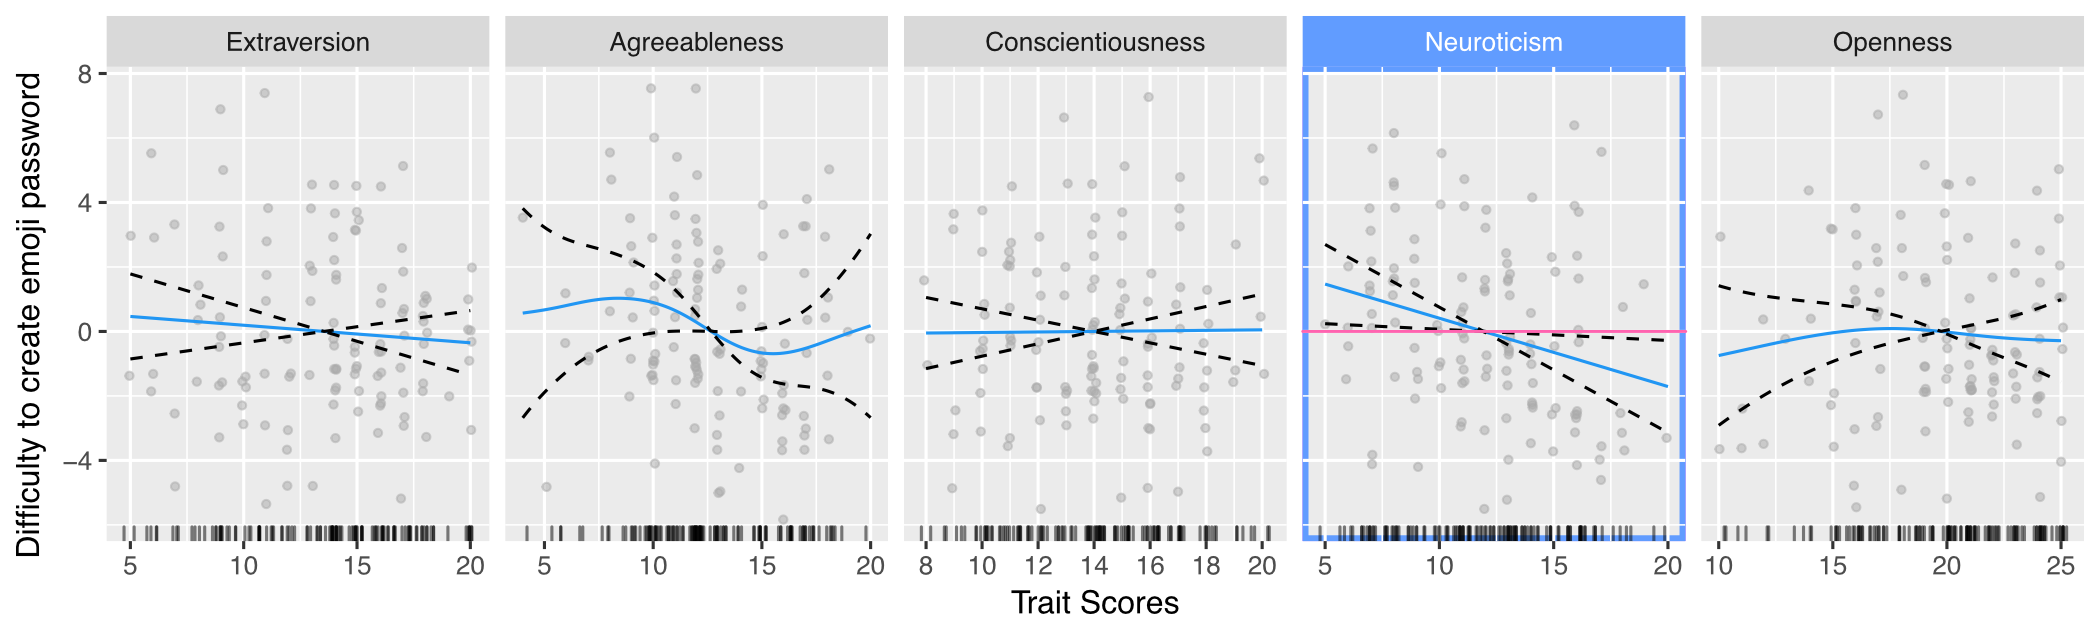
\includegraphics[width=\linewidth]{personality/png/dc-emoji-b5-v2}
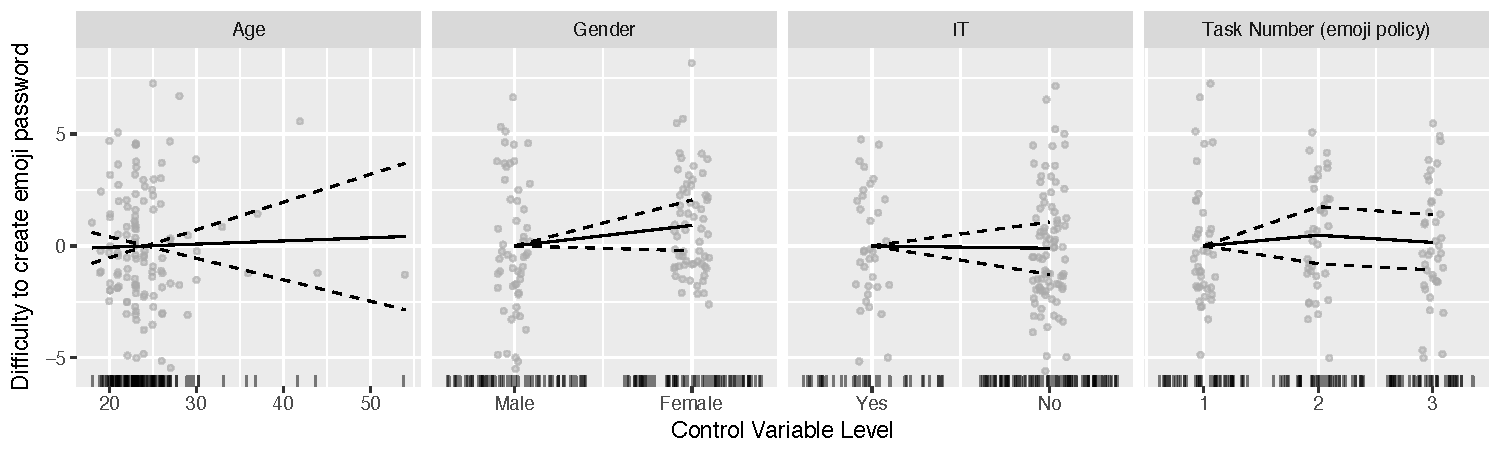
\includegraphics[width=\linewidth]{personality/png/dc-emoji-control-mod-v2}
\caption{\label{fig:personality:dc-emoji-b5}Associations between predictors and \textbf{difficulty} to create a password under the emoji12 policy. Charts visualize the functions derived from the Generalized Additive Models (GAMs). Neuroticism was significantly negatively associated with difficulty (highlighted in blue), i.e. it was easier to create emoji-passwords if participants scored high on neuroticism.}
\end{figure}

\noindent
\fbox{
	\label{sec:personality:study1:how-to-read-diagrams}
	\hspace{0.5cm}
	\centering
	\parbox[t][11.5cm]{0.9\linewidth}{
		\section*{How to Read Smoothed Regression Plots}\label{sec:personality:how-to-read-gam}
		\small
		Figure \ref{fig:personality:dc-emoji-b5} shows the first example of regression plots that will be used throughout the thesis where appropriate. There is a separate plot for each marginal association with a given predictor. The solid curve/line represents the estimated regression curve. If it is a straight line, the association can be modeled linearly (e.g. neuroticism in Figure \ref{fig:personality:dc-emoji-b5}). If it is a ``wiggly'' curve, the association is modeled with polynomial terms of different degrees (e.g. Agreeableness in Figure \ref{fig:personality:dc-emoji-b5}). The model intercept is at $y=0$. In many cases, residuals are plotted at their respective $(x,y)$ position to give a sense of clusters. At the bottom border of the plots, we often add ``rugs'' to show the number of observations/residuals along the x-axis. 
		
		Interpreting the effect size and significant contribution to the model fit is visible in two ways. First, the slope of the fitted line shows estimated strength of associations. Second, there are two dashed curves surrounding the fitted curve/line that visualize 95\% confidence intervals. Both curves are entirely above, respectively entirely below, the intersection between the fitted curve and the intercept at $y=0$, the association is significant at the 0.05 alpha level.
		
		In Figure \ref{fig:personality:dc-emoji-b5}, we highlighted this for the neuroticism plot. Left to the point of intersection, both dashed lines are above the intercept (in pink color); analogously, the dashed lines are below the intercept  on the right-hand side, indicating a significant contribution to the model. 
		
%		\begin{itemize}[leftmargin=*]
%			\item Personality is weakly associated with all the measured dimensions: strength perception, policy preference / usability, and password selection. Most notably openness and neuroticism showed conclusive associationes.
%			\item The models for the perception of passphrases achieved the highest fit, suggesting a predictable association between personality and strength perception for this type of password. Comparing two passwords was associated with the conscientiousness traits. Mixed models that use both password features and personality trait scores as covariates are the most feasible approach.
%			\item Older users might be the best target group for password support tools, because age was a good predictor of their usage. Suggesting good tools during account creation might lead to higher adoption 
%			%			\item Segmentation of users
%			\item Nudges designed for neuroticism should make emotional state more salient and highlight the benefits of \underline{long} passwords. 
%		\end{itemize}
	}
	\hspace{0.5cm}
}

\paragraph{Personality Traits}
Contrarily to the modeling functions for control variables, we mostly observed non-linear associations between trait scores and creation difficulty (see Figure \ref{fig:personality:dc-emoji-b5}).
%emoji personality
One exception is the weak linear association in the emoji12 ($B=-0.22$) condition. It tells us that it was slightly easier to create emoji-passwords for people with higher neuroticism scores. The neuroticism trait is also referred to as ``emotional stability'' \cite{Costa1992NEO}, i.e. neurotic people are usually more emotional. Expressing \textit{emotions} with emojis in passwords seems to support this trait and come easier to users scoring high on neuroticism. %(this is a great result, albeit weak. neurotic people are by defintion more \textit{emotional}, and emojis seem to cater to this trait.)

%agreeableness weak non linear, and interesting curve (up and down) for emoji12
%openness weak non linear, but too little data to conclusively decide. 

% 2word12 personality
%effects not as clear as for the emoji policy. highly open people report slightly less difficulty to create a 2word12 password.
In the models for the 2word12 policy, all associations were non-linear and thus inconclusive at this point. For the 3class12 policy, associations were linear but trivial for the extraversion, conscientiousness, and neuroticism factors. In summary, scores of the ``Creation Difficulty'' scale are difficult to explain with personality traits, but control variables appear to have stronger influence. Only neuroticism is associated notably with difficulty to create an emoji-password.
% 3class12
%linear associations are negligible for extraversion, conscientiousness, and neuroticism. 
%non-linear associations for agreeableness and openness. at value around 15 (from 20) the difficulty seems to increase (hard to interpret this finding). People with agreeableness scores of 18 and greater find it more difficult to create a 3class12 password by up to 1.5 points. Openness is inversely correlated here. the more open the participant was, the more likely they found it easy to create a 3class12 password. 

%%%%%%%%%%%
%%%%%%%%%%% Preference for one policy or another
%%%%%%%%%%%
\subsubsection{Policy Preference}
Table \ref{tab:pws_pers:distribution-binary-ranks} shows the overall preference for the three policies. It is evident that participants generally preferred the 3class12 policy (68\%). The emoji policy was best ranked by 18 participants, and 2word12 by 12 participants. Using logistic additive regression, we can determine the factors that contribute to these preferences. %https://web.stanford.edu/~hastie/Papers/AdditiveLogisticRegression/alr.pdf
In essence, the model gives us the likelihood of voting a given policy to the top, which is a binary decision (1 = preferred, 0 = not preferred). 
%did policy X land on top spot ? yes = 1, no = 1. thus, no encompasses the two other options.
%Logit model. 
\begin{table}
	\centering
	\caption{\label{tab:pws_pers:distribution-binary-ranks} Distribution of binary rankings of the three available policies. Evidently, 3class12 was ranked best in most cases. }
	\begin{tabular}{llll}
		~ 			& emoji12	& 2word12 	& 3class12 \\ \hline\hline
		1st rank	& 18		& 12		& 67 \\
		other rank 	& 80 		& 85 		& 31 \\ \hline
		n			& 98		& 98		& 98		 
	\end{tabular}
\end{table}

% predictors: demography and structure
Including demographic control variables as predictors, we observed strong effects for IT-background. The probability of putting emoji12 at the top is $exp(B{emoji-IT}) = 9.87$ for participants without technical background, so around ten times higher. Only one respondent with an IT background ranked emoji12 on the top. %This fits the finding that non-IT people found it easier to create an emoji12 password.
% order of policies 
The order in which policies were displayed also produced a notable effect. If emoji12 was part of the second $exp(B_{emoji-pos2}) = 0.27$ or third task $exp(B_{emoij-pos3}) = 0.76$, the likelihood to rate it the best policy slightly decreases. Other task orders, as well as age-related preferences, were inconclusive.

% personality
As with creation difficulty, rank-associations with personality traits were generally weak. The likelihood to prefer 2word12 decreased with higher extraversion scores $exp(B_{2word12-E}) = 0.82$. High agreeableness scores entailed higher chances to vote for emoji12 $exp(B_{emoji12-A}) = 1.28$. Interestingly, only very high neuroticism scores (>17) caused a  stark increase in favoring the emoji policy. However, the sample is thin in this area so the model is more unstable at this boundary. Other associations were negligible or inconclusive. 
%for agreeableness both linear and non-linear effects are visible; openness or conscientiousness have negligible, random associations. for neuroticism we lack data in edge cases (low or high trait scores) to draw conclusions. %there are more results in the BA, but I do not really see the point of reporting all the details of inconclusive results

%%%%%%%%%%%
%%%%%%%%%%% Password selection -- mostly emoji histogram
%%%%%%%%%%%
%\subsubsection{Password selection}

%\todo{create a emoiji selection histogram}. In essence, some emoji were strongly preferred, e.g. the red heart and the ``pouting face''. analyze: what were the usability ratings/rankings of those who picked the heart vs. the pouting face, i.e. are emojis with a positive connotation used by people who are happy that they can select an emoji password? I guess there are significant effects here. 

%TODO look into timings -- did conscientious people take longer to generate passwords?

\subsubsection{Time to Create Passwords}
The second usability metric was the time the participants took to create passwords. It can also be interpreted as \textit{effort} put into the task. The most interesting associations were visible for the 3class12 policy, where all personality traits could be modeled as linear predictors (see Figure \ref{fig:personality:timing-3class-b5}), and all showed medium-strong correlations (details in the Appendix, Table \ref{tab:personality:study-1:timing-models}). One might have suspected that conscientious people would invest more time, because one of their common attributes is diligence. However, this was not the case: conscientiousness was negatively associated with creation time for all policies ($B_{emoij12-C}=-3.58,B_{2word12-C}=-3.4,B_{3class12-C}=-2.09$). Neuroticism was significantly negatively associated with creation time, while agreeableness was marginally positively associated in 3class12. Demographic control factors indicated that, on average, women spent more time creating passwords in all conditions ($W=1166$, \pvallt{0.01}). The biggest effects were visible for task number as predictor: our participants took significantly less time to select passwords for the second and third tasks (example shown in \ref{fig:personality:timing-2word-control}). Most likely, this is a learning effect or due to people modifying their previous passwords. 


\begin{figure}
	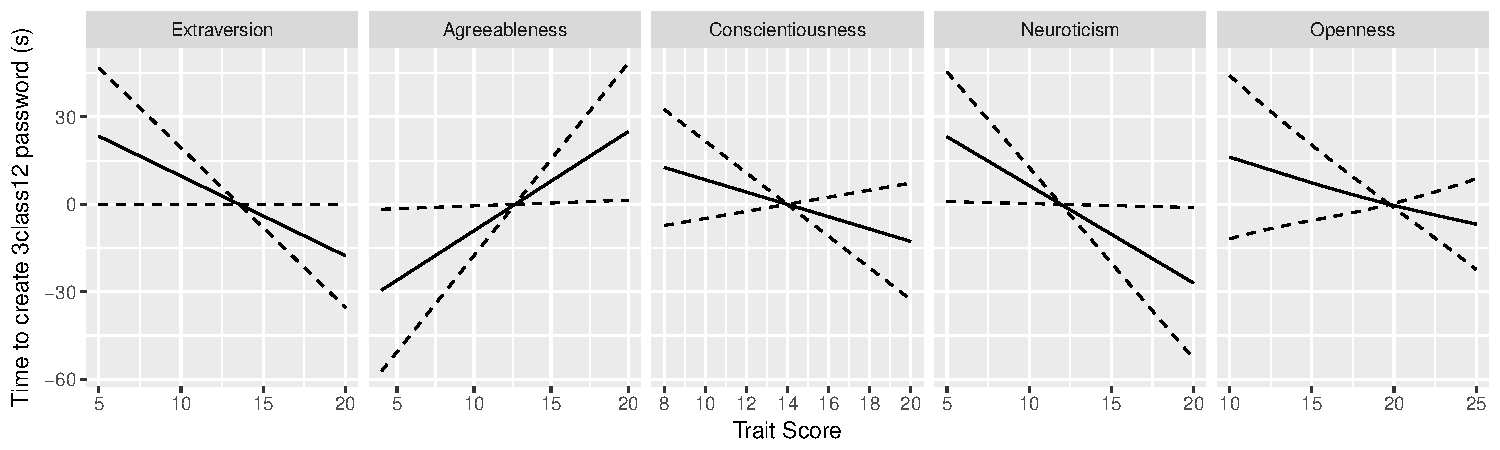
\includegraphics[width=\linewidth]{personality/timing-3class-b5}
	\caption{\label{fig:personality:timing-3class-b5}Associations between personality traits and time to create a 3class12 password. All traits could be modeled as linear predictors.}
\end{figure}

\begin{figure}
	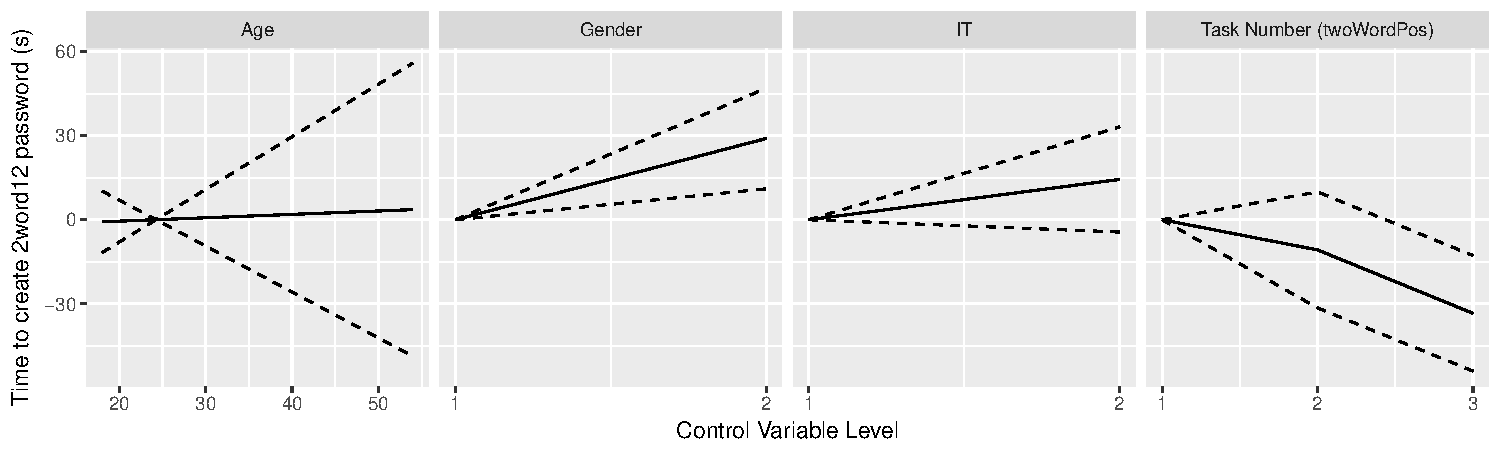
\includegraphics[width=\linewidth]{personality/timing-2word-control}
	\caption{\label{fig:personality:timing-2word-control}Associations between control variables and time to create a 2word12 password. Especially the task number and gender were showed strong associations.}
\end{figure}


%TODO the qualitative and plain-text passwords data is also interesting but goes too far at this point. 

\subsection{Finding Summary}
Overall, the usability metrics were comparable for all policies and the ranking was fairly homogeneous. So, any deviance from the mean could potentially be explained by personality traits and other confounding factors. In terms of personality, the most important finding was that scores on the neuroticism dimension seem to be positively associated with the usability of the emoji policy. As indicated above, emojis in passwords appear to fulfill their purpose in that they help some people express their emotions. Participants who did not have a background in IT were much more likely to prefer the emoji policy, and their neuroticism score played a subordinate role. Perhaps, a lack of expertise does not allow those participants to consider the switch from keyboard to mouse and vice versa (\textit{homing}). Moreover, the 3class12 policy received the most votes which might be due to the \textit{status quo bias} or \textit{familiarity bias}. 3class12 is the only commonplace policy among the tested ones, so participants were already used to it and voted it first. The timings were mostly affected by the task order -- participants spent less time on the second and third creation task. So although personality traits serve as predictors for timings, these effects were weaker by comparison. 

In summary, control factors had a greater effect on password usability and approval of policies than personality traits. Nonetheless, medium to strong effects are more likely to be detected with our sample size to begin with. So, the fact that we even observed small associations indicates that personality is a contributing factor to the perception of password policies. At this stage of the research we were not able to look into the selection behavior because the repeated measures design stood in the way. Thus, we designed and conducted two further studies to investigate the effect of personality on password strength perception and selection. 

%It could have been useful to include a recall test à la ``which passwords do you still remember after filling out the personality questionnaire?'' 

%medium associations between extraversion, agreeableness, and neuroticism (basically the other three dimensions that were not useful before), but control variables are associated to a larger degree.
%emoji policy similar results as traditional policies, i.e. it is wortwhile to experiment with it

%TODO re-read the discussion section, because the findings are a bit higher level and more understandable


%non linear associations probably explicable by other variables, e.g. intercorrelation -- 
%todo{discuss the personality traits and associations, try to explain them.}

%demographics play a role - (careful now, cowboy): policies could be tailored to gender. but i'm kind of reluctant to put this argument forward. at least IT background could be considered a factor for the policy. a personalized policy would make it more difficult for horizontal attacks because the policy is unpredictable.

%mutually exclusive effects for ranking are clear because of the binary nature.

%wild idea: if positioning influences the favorability of policies, one could leverage this. like anchoring and decoy (chose your own policy of the three). commitment and consistency as well (commit to your policy, create a strong password to be consistent with your commitment.)

%%%%%%%%%%%%%%%%%%%%%%%%%%%%%%%%%%%%%%%%%%%
%%%%
%%%%
%%%%			STUDY  2 TWO ZWEI
%%%%			PERCEPTION
%%%%
%%%%
%%%%%%%%%%%%%%%%%%%%%%%%%%%%%%%%%%%%%%%%%%%
\section{Study 2: Strength Perceptions}
With an observational online study, we explored the associations between psychological variables and password strength perception. We regard the perception of strength as necessary step before looking at actual behavior, which is more difficult to observe. Hence, we tried to find associations between subjective password strength ratings and scores on well-established psychometric scales. Before we ran the study, we pre-registered the experiment with the open-science framework (OSF)\footnote{\url{https://osf.io/}, last accessed 11.09.2016} and conducted all analyses as predicted to mitigate confirmation bias. Since we consider our research efforts mostly exploratory, we approached the study without specific hypotheses regarding the influence of certain personality traits or decision making styles on the perception of password strength.

\subsection{Structure}
% DEMOGRAPHICS
The study was divided into six parts of which two were standard psychometric tests. After a brief introduction where the participants were informed about the background of the study, they answered basic demographic questions about gender, age, educational and professional background. %This information is important for the ratings on the password scales, because advanced knowledge in IT(-security) may lead to a different rating than the general audience. 

% META STATISTICS / CREATION
The second part was about collecting characteristics about the passwords that our participants used on real online accounts. Here, we asked about typical password attributes, like LUDS (lower-, uppercase, digits, symbols), length and the inclusion of dictionary words. The collection of such password descriptions is an ethically reasonable way to study actual behavior that does not directly involve creating and disclosing an entire password \cite{VonZezschwitz2013SurvivalShortest}. Participants could select from a list of accounts that they used on a regular basis, e.g. Facebook, YouTube, Netflix, Google. If they did not have any of the selectable accounts they could provide another. The description of a participant's password is called \textit{meta password} in the remainder of the paper. 
%TODO entscheiden ob das reinkommt Additionally we had them create a password which they would rate as sufficient to protect such an online account and that is memorable. We asked not to enter a password that they were currently using. At the end of the study, we again inquired after the fictional password to measure short-term memorability. 


%%% TABLE: PASSWORDS
\begin{table}[htbp]
  \centering
  \caption{Set of passwords that we divided into different length and strength categories (as measured with zxcvbn). Features: U = uppercase, D = digits, S = symbols}
 % \small
    \begin{tabular}{lllcccr}
    \multicolumn{1}{c}{\multirow{2}[1]{*}{Password}} & \multicolumn{2}{c}{Categories} & \multicolumn{3}{c}{\multirow{2}[1]{*}{Features}} & \multicolumn{1}{c}{guesses} \\
      & Length & Strength & \multicolumn{3}{c}{} & \multicolumn{1}{c}{(log10)} \\
    \midrule
    hagrqqqqthhbbe & Long & Strong & \multicolumn{3}{c}{-} & 12.48 \\
    etuhcarap & Short & Weak & \multicolumn{3}{c}{-} & 4 \\
    AbWxCdYz & Short & Medium & \multicolumn{3}{c}{U} & 8 \\
    1qaz2wsx3edc & Long & Weak & \multicolumn{3}{c}{D} & 3 \\
    a6a4ba8a & Short & Medium & \multicolumn{3}{c}{D} & 8 \\
    ieatkale88 & Short & Medium & \multicolumn{3}{c}{D} & 10 \\
    thedzfhg123 & Short & Medium & \multicolumn{3}{c}{D} & 10 \\
    11Nd1sPPut8ble99 & Long & Strong & \multicolumn{3}{c}{U,D} & 16 \\
    bicycles-peaches-cold & Long & Strong & \multicolumn{3}{c}{S} & 13.69 \\
    AatIcs,ijayl-t & Long & Strong & \multicolumn{3}{c}{U,S} & 13.95 \\
    p@ssw0rd & Short & Weak & \multicolumn{3}{c}{D,S} & 0.95 \\
    ocean4 Size !beer Car & Long & Strong & \multicolumn{3}{c}{U,D,S} & 20.39 \\
    F@m1Ly07\% & Short & Medium & \multicolumn{3}{c}{U,D,S} & 6.88 \\
    \bottomrule
    \end{tabular}%

  \label{tab:password-list}%
  
\end{table}%

%  RATING
In the third part of the study, the \textit{rating part}, the participants assessed the strength of one password at a time in random order. The passwords had to be rated on 7-point scales ranging from \textit{1 = very weak} to \textit{7 = very strong}. We picked a set that was comparable to related work \cite{Ur2016PerceptionsPassword} and that we carefully designed around certain attributes. Table \ref{tab:password-list} shows the selected set of passwords and their features. The ``length'' category distinguishes between short passwords with nine characters or less and long passwords with ten characters or more. The distinction is inspired by real-world policies that usually require nine or more characters \cite{Wang2015EmperorsPolicies}. Other passwords are usually ``below that bar'' and can thus be considered too short. The ``strength'' category groups passwords on three levels by their objective guessability as measured by zxcvbn. Weak passwords require less than $10^{6}$ guessing attempts, strong passwords at least $10^{12}$ guesses, and medium passwords anything in between. This classification is in concordance with related work \cite{Florencio2014AdministratorsGuide, Wheeler2016zxcvbn} . To fully counterbalance all category combinations, one would require 120 items, which we could not implement for the sake of brevity. Hence, we kept the number of items small to mitigate fatigue during the study sessions. In the chosen set of 13 passwords, there were at least three items for each distinct category, i.e. three short, long, weak and strong passwords, and at least three passwords containing at least one of LUDS features (lowercase, uppercase, digits and symbols)

% COMPARISON
Following a similar procedure as Ur et al. \cite{Ur2016PerceptionsPassword}, participants moved on to compare the strength of passwords pairs (\textit{comparsion part}). The 7-point scale ranged from ``<left password> is much stronger'' to ``<right password> is much stronger''. The pairs were constructed such that the passwords differed, e.g., in the existence and positions of digits and uppercase letters. Figure \ref{fig:comparisontask} illustrates our scoring schema. 

\begin{figure}
	\centering
	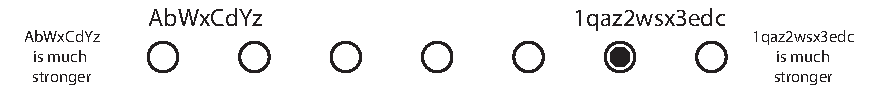
\includegraphics[width=\linewidth]{figures/comparisontask}
	\caption{\label{fig:comparisontask} Simplified item of the comparison task. The passwords differ in length, strength, and the usage of uppercase letters and digits. Here would have scored the importance of length and digits with +2 while the importance of strength and uppercase letters was scored with -2.}
\end{figure}

If the passwords measurably differ in strength as in Figure \ref{fig:comparisontask}, the ratings show if the participants' perceptions match reality. In total, ten comparisons had to be made in random order, in which we permuted the combinations. For this task, we also added an attention check where the passwords on both sides of the scale matched, allowing us to exclude responses where the answer differed from ``both passwords are equally strong''. 

Next, we requested self-assessment about security-related behavior using the Security Behavior Intentions Scale (SeBIS) \cite{Egelman2015SeBIS}. This scale comprises the dimensions \textit{securement}, \textit{passwords}, \textit{awareness}, and \textit{updating}. For each dimension, a score is calculated with four items totaling up to 16 additional items in our study. However, in discussions after the experiment we received hints that it would have been better to include a gap of a couple of days before collecting the SeBIS data to ensure its validity. Since we failed to take this into account beforehand, we do not report the results further, but it is important to mention that the questionnaire included 16 additional items. 
%The items are phrased as statements to which respondents can indicate how often they show a certain type of security-related behavior. The scale ranges from \textit{1 = never} to \textit{5 = always}. The \textit{password} dimension measures general attitude towards passwords, which we can utilize to inform our interpretation later.

The study concluded with two psychometric tests. In the \textit{Big-Five part}, we utilized a set of 50-items from the International Personality Item Pool (IPIP), which is a representation of Costa and McCrae's NEO-PI-R domains \citep{Costa1992NEO}\footnote{All items of the personality test can be found here: \url{http://ipip.ori.org/newNEODomainsKey.htm}, psychometric properties: \url{http://ipip.ori.org/newNEO_DomainsTable.htm}}. In this personality test, participants rate how accurately a certain statement portraying a certain personality characteristic describes themselves. Each item is a 5-point scale with the labels \textit{very inaccurate, moderately inaccurate, neither accurate nor inaccurate, moderately accurate, very accurate}. Every personality trait is tested with five positively and five negatively keyed items. It was shown that the 50-item version of the test shows high correlation with more exhaustive tests ($r > 0.75$ in all dimensions) and is thus a sufficiently reliable test. We randomized the order of the items.

Egelman and Peer found that the general decision making style had higher predictive power than the Big-Five traits for privacy-related behavior \cite{Egelman2015AverageUser}. Thus, we wanted to test the feasibility of both psychometric tests and finished the study with the \textit{GDMS part}. This scale uses 25 positively keyed items to measure the five decision-making styles \textit{rational}, \textit{intuitive}, \textit{dependent}, \textit{avoidant} and \textit{spontaneous}. 

\subsection{Quantitative Analysis}
We used a set of statistical tests to explore the relationship between the scores psychometric scales and password strength perception. Since at least three passwords showed a certain characteristic, e.g. uppercase letters, we averaged the ratings for them accordingly. Moreover, in the psychometric tests we accounted for negatively keyed items, i.e. those items that were phrased with negations like \textit{``I don't talk a lot''}. We inverted the ratings where necessary and afterwards calculated the sum of agreement for each dimension. 

We use linear regression with subjective password strength assessments as dependent variables. We calculate one score per participant and password category by averaging the corresponding ratings. Psychometric test results on sub-scales served as independent variables. We always control the regression models for gender, technical background and education level to prevent misinterpreting the effects. Education was coded as ordinal variable from 1 (grammar school) to 7 (professional degree like PhD, MD, JD). We check for collinearity using variance inflation factors (VIF) and only retain factors with VIFs close to 1 \cite[p. 217]{Weisberg2005applied}. Also, because of the exploratory nature, we can use step-wise regression methods to build the models. To mitigate type-II errors herein, we use a backward approach \cite[p. 161]{Field2005DiscoveringStatistics} and exclude factors that do not improve the model significantly. Finally, we perform Durbin-Watson tests to rule auto-correlation effects (target value $d=2$). While p-values do not add much to the interpretability of the findings, we report them for the sake of completeness.  
%TODO Quelle!
%Our level for statistical significance is $\alpha = 0.05$, unless Bonferroni correction requires a lower value. 

When we report the results of linear regression models, we only do so for the models with the highest adjusted $R^2$ value, i.e. the model where the number of predictors leads to the best model-fit explaining the variance in the dependent variable. The values in Tables \ref{tbl:personalpw_regression} through \ref{tab:Comparison-Regression} are the \textbf{standardized beta} correlations, i.e. they are unit-less and lie between -1 and +1. 

\subsection{Qualitative Analysis}
To better understand the reasoning behind the ratings and comparisons, we also inquired how the respondents approached the rating task. They could enter free-text answers after all ratings were done. The answers were then coded independently by two members of the team. The first coding step was to find categories and propose the code book. Afterwards, the proposed codes were handed over to the second coder, who sorted answers into the categories and amended new ones where necessary. Interrater agreement between the two coders was satisfactory (78\%, Krippendorff's $\alpha = 0.55$) and the final the code book could be created after discussing the discrepancies. We report how many participants mentioned a particular theme in their response regarding their rating strategies.


\subsection{Recruitment}
We utilized the online research platform Prolific\footnote{\url{https://prolific.ac}, accessed 01.09.2016} to administer our survey. Participants received \$2.65 upon successful completion, which took 20 minutes in average. This compensation level is suggested as part of the ethical reward guidelines on the platform. Only an English-speaking audience was eligible to participate. From the 178 people who started the survey, 104 finished it. To prevent low quality answers, we introduced an attention check during the comparison part of the experiment.  

%In the first phase of the study, the participants were asked to imagine their email provider required them to create a new password and they could not select their current one. This measurement was taken early to prevent bias from showing different types of passwords. The answers were collected in plain text. We proceeded to have the users choose the type of account that they would be willing to secure with their selected password in the real world. This would indicate the effort and the value of their selection.


\subsection{Ethical Considerations}
There is no institutional review board for this kind of studies at our institution. However, we designed the questionnaire to respect the participants' privacy and did our best to minimize the level of disclosure of sensitive data. The metrics we collected to characterize the participants' passwords are most likely insufficient to reconstruct the passwords in a straightforward way and can thus be considered ethically acceptable. 


\subsection{Limitations}
%It is good to discuss the limitations before the results. Thus, the reader can bear them in mind when they are reading on. 

Like most studies involving personality assessment, the result is only a rough model of a person's personality and does not include all facets. We chose a test with 50 items to assess the Big-Five traits. While such psychometric tests exist with item counts between 10 \cite{Gosling2003TIPI} and 240 items \cite{Costa1992NEO}, the 50-item version has high internal reliability and does not fatigue the respondents as much as more exhaustive tests. Additionally, with a sample size of 100 participants, power-analysis tells us, that only strong and medium interactions are likely to be found for with our regression models (cf. \cite{Shevlin1998SampleSize} or \cite[p. 223]{Field2005DiscoveringStatistics}). At this stage of the exploration, however, this is what we aimed for. If we do find effects with such a small sample, then they must be large enough to justify follow-up investigations with larger samples. 

Furthermore, the methodology relies on self-assessment and honest answers, which are difficult to control. We introduced an attention check to mitigate the problem, by asking people to compare two identical passwords. For the meta-password, we do not know whether it was created on a mobile or desktop device. Passwords created on mobiles are usually less complex than those created on desktops \cite{Melicher2016UsabilityMobileTextPasswords, VonZezschwitz2014HoneyIShrunkTheKeys}. 

We also have to be careful not to over-generalize the results due to our use of crowd-sourced study participation. The responses may not be representative for a larger population, e.g. because the sample stems from a technically savvy audience. Users registering for tools like Prolific or Amazon Mechanical Turk may also have stronger financial motivation to do so than the rest of the population \cite{Ross2010WhoAreTurkers}. 

Finally, the study set-up and procedure may also influence the interpretability of the outcome. We decided not to randomize the order of the question blocks to maintain full control over the general procedure. When we measure dependent variables, the order of questions is still randomized in the question groups. This way, the potential fatigue effects are the same for all participants at the different stages, while the important questions are in random order. Moreover, the items for password pairs were not fully counterbalanced on all levels to prevent fatigue when answering the entire questionnaire. A more exhaustive set of tested passwords would increase the generalizability. 

%we need to be aware that a more faceted personality profile may reveal larger differences. 
%TODO viele antworten deuteten darauf hin, dass englisch nicht in die muttersprache ist. 
%TODO meta password characteristics are not an accurate proxy for password strength, as depicted in the background section. 
%Our proxy for password strength is the result of the zxcvbn estimator algorithm \cite{Wheeler2016zxcvbn}. While it can estimate the strength of passwords in attack scenarios up to one million guesses, its estimates become more fuzzy above this threshold. However, for the purpose of the study, the estimate was considered good enough as it still highly correlates with the estimates of more sophisticated tools like the password guessing service (PGS) \cite{Ur2015MeasuringRealWorldAccuracies}. 
%\begin{itemize}
%\item we might measure intelligence
%\item self-reporting might not be accurate
%\end{itemize}


%As we collected plain text passwords that could -- in theory -- be linked backed to an individual, we took special care to point out that participants should not enter their actual password, but to think of a new one. The additional meta characteristics are most likely insufficient to reconstruct a participant's actual password. 

\begin{figure}
	\centering
	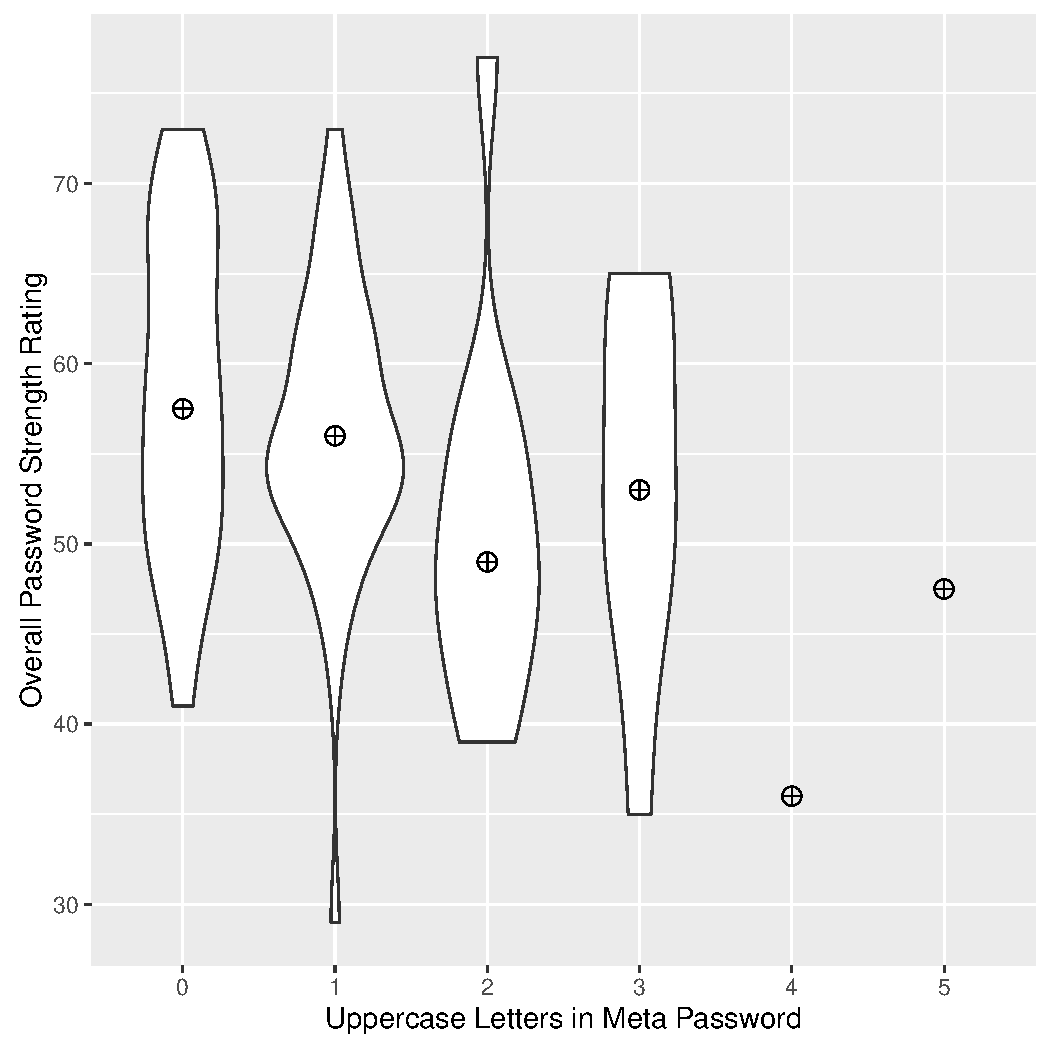
\includegraphics[width=\linewidth]{figures/MetaPW-Violinplot}
	\caption{\label{fig:MetaPW-ViolinPlot} Violin plot of strength ratings, grouped by the number of uppercase letters in the participants' meta password. The plot gets broader, the more respondents scored in the particular range. The plot shows a negative association between overall password strength and uppercase letters in the meta password.}
\end{figure}



%%%%%%%%%%%%%%%%%%%%%%%%%%%%%%%%%%%%%%%%%%%
%%%%
%%%%
%%%%			RESULTS 
%%%%
%%%%
%%%%%%%%%%%%%%%%%%%%%%%%%%%%%%%%%%%%%%%%%%%
\subsection{Results}
In this section, we first describe the participants and meta password characteristics before we proceed to the regression analyses. The final part of this section shows qualitative findings and a brief synthesis of the results. 

\subsubsection{Participants}
We collected 104 complete samples. We had to remove three samples from respondents who failed the attention check. Another response was removed because all responses on point scales were answered with the same value. This procedure is proposed by the IPIP project \footnote{\url{http://ipip.ori.org/newValidity.htm} accessed 02.09.2016}. The resulting total N = 100 was divided into 42 female and 58 male participants. Their average age was 28 years ($Standard Deviation~(SD) = 9,~Minimum = 16,~Maximum = 61,~Median~(Md) = 26$). 44 responses came from students. The education level was high with 59 participants reportedly having a bachelor's (44) or master's (15) degree. 29 participants claimed to have a computer science or IT-related background. In summary, our sample stems from a young, educated and fairly technically savvy population. This convenience sample is not ideal, but we hope to deal with this skew by including demographics as predictors in the regression models.

\subsubsection{Strength Categories and Meta Passwords}
On average, the respondents correctly identified weak, medium and strong passwords in the rating task, i.e. their perception matched reality. The average scores were $M=3.60~(SD=1.07)$ for weak, $M=4.25~(SD=0.95)$ for medium and $M=4.71~(SD=0.90)$ for strong passwords. A Friedman rank test showed that these ratings differed significantly ($F(2)=59.91,~p < 0.001$). 

%%%%%% TABLE 
\begin{table*}%[h!tbp]
  \small
  \centering
  \caption{Regression analysis for password ratings in different categories as dependent variables and psychometrics as independent variables variables. Demographic data serves as control variables. Numbers in bold indicate statistical significance ($p<0.05$). The Big-Five factors had higher predictive value and than the GMDS factors.}
    \resizebox{\linewidth}{!}
{
\begin{tabular}{rl|r|rr|rrr|rrr}
    \multicolumn{2}{l|}{Predictor} & \multicolumn{1}{l|}{Overall} & \multicolumn{1}{l}{Short} & \multicolumn{1}{l|}{Long} & \multicolumn{1}{l}{Weak} & \multicolumn{1}{l}{Medium} & \multicolumn{1}{l|}{Strong} & \multicolumn{1}{l}{Symbols} & \multicolumn{1}{l}{Digits} & \multicolumn{1}{l}{Uppercase} \\
\cmidrule{3-11}    \rowcolor[rgb]{ .718,  .871,  .91} \multicolumn{1}{l}{Big Five} & Neuroticism & \cellcolor[rgb]{ 1,  1,  1}  & \cellcolor[rgb]{ .949,  .91,  .518} 0.15 & \cellcolor[rgb]{ .949,  .91,  .518} 0.15 & \cellcolor[rgb]{ .969,  .914,  .518} 0.14 & \cellcolor[rgb]{ 1,  1,  1}  & \cellcolor[rgb]{ .98,  .627,  .459} -0.15 & \cellcolor[rgb]{ 1,  1,  1}  & \cellcolor[rgb]{ 1,  1,  1}  & \cellcolor[rgb]{ 1,  1,  1}  \\
    \rowcolor[rgb]{ .718,  .871,  .91}   & Openness & \cellcolor[rgb]{ .976,  .518,  .439} \textbf{-0.25} & \cellcolor[rgb]{ .976,  .541,  .443} \textbf{-0.23} & \cellcolor[rgb]{ .98,  .573,  .447} \textbf{-0.2} & \cellcolor[rgb]{ .976,  .498,  .435} \textbf{-0.27} & \cellcolor[rgb]{ .98,  .616,  .459} -0.16 & \cellcolor[rgb]{ .98,  .604,  .455} -0.17 & \cellcolor[rgb]{ .984,  .647,  .463} -0.13 & \cellcolor[rgb]{ .976,  .541,  .443} \textbf{-0.23} & \cellcolor[rgb]{ .984,  .639,  .463} -0.14 \\
    \rowcolor[rgb]{ .718,  .871,  .91}   & Agreeableness & \cellcolor[rgb]{ .898,  .894,  .514} 0.18 & \cellcolor[rgb]{ .949,  .91,  .518} 0.15 & \cellcolor[rgb]{ .898,  .894,  .514} 0.18 & \cellcolor[rgb]{ .898,  .894,  .514} 0.18 & \cellcolor[rgb]{ 1,  1,  1}  & \cellcolor[rgb]{ .969,  .914,  .518} 0.14 & \cellcolor[rgb]{ .984,  .918,  .518} 0.13 & \cellcolor[rgb]{ .996,  .91,  .514} 0.11 & \cellcolor[rgb]{ 1,  1,  1}  \\
    \rowcolor[rgb]{ .988,  .835,  .706} \multicolumn{1}{l}{GDMS} & Rational & \cellcolor[rgb]{ 1,  1,  1}  & \cellcolor[rgb]{ 1,  1,  1}  & \cellcolor[rgb]{ 1,  1,  1}  & \cellcolor[rgb]{ 1,  1,  1}  & \cellcolor[rgb]{ 1,  1,  1}  & \cellcolor[rgb]{ 1,  1,  1}  & \cellcolor[rgb]{ 1,  1,  1}  & \cellcolor[rgb]{ 1,  1,  1}  & \cellcolor[rgb]{ .984,  .918,  .518} 0.13 \\
    \rowcolor[rgb]{ .988,  .835,  .706}   & Intuitive & \cellcolor[rgb]{ 1,  1,  1}  & \cellcolor[rgb]{ 1,  1,  1}  & \cellcolor[rgb]{ 1,  1,  1}  & \cellcolor[rgb]{ 1,  1,  1}  & \cellcolor[rgb]{ 1,  1,  1}  & \cellcolor[rgb]{ 1,  1,  1}  & \cellcolor[rgb]{ 1,  1,  1}  & \cellcolor[rgb]{ 1,  1,  1}  & \cellcolor[rgb]{ .996,  .898,  .51} 0.1 \\
    \rowcolor[rgb]{ .988,  .835,  .706}   & Avoidant & \cellcolor[rgb]{ 1,  1,  1}  & \cellcolor[rgb]{ 1,  1,  1}  & \cellcolor[rgb]{ 1,  1,  1}  & \cellcolor[rgb]{ .984,  .639,  .463} -0.14 & \cellcolor[rgb]{ 1,  1,  1}  & \cellcolor[rgb]{ 1,  1,  1}  & \cellcolor[rgb]{ .984,  .647,  .463} -0.13 & \cellcolor[rgb]{ 1,  1,  1}  & \cellcolor[rgb]{ 1,  1,  1}  \\
    \rowcolor[rgb]{ .988,  .835,  .706}   & Spontaneous & \cellcolor[rgb]{ 1,  1,  1}  & \cellcolor[rgb]{ 1,  1,  1}  & \cellcolor[rgb]{ 1,  1,  1}  & \cellcolor[rgb]{ 1,  1,  1}  & \cellcolor[rgb]{ .984,  .918,  .518} 0.13 & \cellcolor[rgb]{ 1,  1,  1}  & \cellcolor[rgb]{ .949,  .91,  .518} 0.15 & \cellcolor[rgb]{ 1,  1,  1}  & \cellcolor[rgb]{ 1,  1,  1}  \\
      & Education &   & \cellcolor[rgb]{ .914,  .898,  .514} 0.17 &   & \cellcolor[rgb]{ .984,  .918,  .518} 0.13 & \cellcolor[rgb]{ 1,  .922,  .518} 0.12 &   &   & \cellcolor[rgb]{ .933,  .902,  .514} 0.16 &  \\
      & CS Background & \cellcolor[rgb]{ .984,  .647,  .463} -0.13 &   & \cellcolor[rgb]{ .984,  .647,  .463} -0.13 &   & \cellcolor[rgb]{ .98,  .627,  .459} -0.15 & \cellcolor[rgb]{ .984,  .682,  .471} -0.1 &   & \cellcolor[rgb]{ .984,  .682,  .471} -0.1 &  \\
    \midrule
      & F & 4.23 & 2.83 & 3.54 & 3.46 & 1.9 & 2.48 & 1.91 & 2.52 & 1.19 \\
      & df & 3 & 4 & 4 & 5 & 4 & 4 & 4 & 4 & 3 \\
      & p & < 0.01 & < 0.05 & < 0.05 & < 0.01 & > 0.1 & < 0.05 & > 0.1 & < 0.05 & > 0.1 \\
      & R$^2$ & \cellcolor[rgb]{ .761,  .898,  .804} 0.12 & \cellcolor[rgb]{ .788,  .91,  .827} 0.11 & \cellcolor[rgb]{ .733,  .886,  .78} 0.13 & \cellcolor[rgb]{ .675,  .863,  .729} 0.15 & \cellcolor[rgb]{ .906,  .957,  .929} 0.07 & \cellcolor[rgb]{ .82,  .922,  .855} 0.1 & \cellcolor[rgb]{ .906,  .957,  .929} 0.07 & \cellcolor[rgb]{ .82,  .922,  .855} 0.1 & \cellcolor[rgb]{ .988,  .988,  1} 0.04 \\
      & Adjusted R$^2$ & \cellcolor[rgb]{ .706,  .875,  .757} 0.09 & \cellcolor[rgb]{ .776,  .906,  .82} 0.07 & \cellcolor[rgb]{ .706,  .875,  .757} 0.09 & \cellcolor[rgb]{ .635,  .847,  .698} 0.11 & \cellcolor[rgb]{ .882,  .949,  .91} 0.04 & \cellcolor[rgb]{ .812,  .918,  .851} 0.06 & \cellcolor[rgb]{ .918,  .961,  .941} 0.03 & \cellcolor[rgb]{ .812,  .918,  .851} 0.06 & \cellcolor[rgb]{ .988,  .988,  1} 0.01 \\
    \bottomrule
    \bottomrule
    \end{tabular}%
}
  \label{tab:Regression-Rating}%
\end{table*}%

%%%%%%%%%%%%%%%%%%%%%%%%%%
%%% 
%%% 		STRENGTH RATING
%%% 
%%%%%%%%%%%%%%%%%%%%%%%%%%
\subsubsection{Standalone Strength Rating}
Our next step was to analyze associations between personality, respectively decision making style and password perception. After having done all required assumption checks, including internal consistency analysis of the scales ($\alpha_{IPIP}=0.72, \alpha_{GDMS}=0.8$), we built regression models containing the scores on the big-five subscales, the GMDS scores and control variables. The initial model hence included the independent variables \textit{openness, conscientiousness, extraversion, agreeableness, neuroticism}, as well as the \textit{rational, intuitive, dependent, avoidant, spontaneous} decision making scores. We added gender, IT-background and education level as controlling factors. The initial model contained all factors and was refined in a backward stepwise removal approach, leaving only those factors with highest predictive values. 

Table \ref{tab:Regression-Rating} shows the regression results of standalone password ratings. The overall ratings in the first column, which we consider the most important metric, were negatively associated with the \textit{openness} trait ($\beta = -0.25, p < 0.05$) (see also Figure \ref{fig:openness-scatterplot}). In other words, participants with higher openness scores were generally more pessimistic regarding password strength, which was also the case if participants had a technical background, albeit this association was not as strong. Higher agreeableness scores were slightly associated with more optimistic overall password ratings. Interestingly, with conscientiousness and extraversion, two of the big-five factors never played a significant role and thus are omitted in Table \ref{tab:Regression-Rating}.

The decision making style predictors were retained in four of the nine models, but never showed high predictive power. Contrarily, the openness trait was retained in the regression models across the board. For example, especially the weaker passwords receive lower ratings from people with higher openness scores. However, the average adjusted $R^2$ across all categories tells us that the models explain only a rather small portion of the variance in the password ratings ($M=0.06~(SD=0.03)$). 

%The lower half of Table \ref{tab:B5-Regression-Comparison} shows the analysis results for standalone password ratings. One can see that there were no striking associations between predictors and dependent variables. Also, the models with the highest $R^2$ value needed six degrees of freedom on average. This means that no particular decision making style stands out to inform the predictions. The maximum $R^2$ value across the models here is $0.05$, i.e. very low. Thus, decision making style did not explain variances satisfactorily.

\begin{figure}
	\centering
	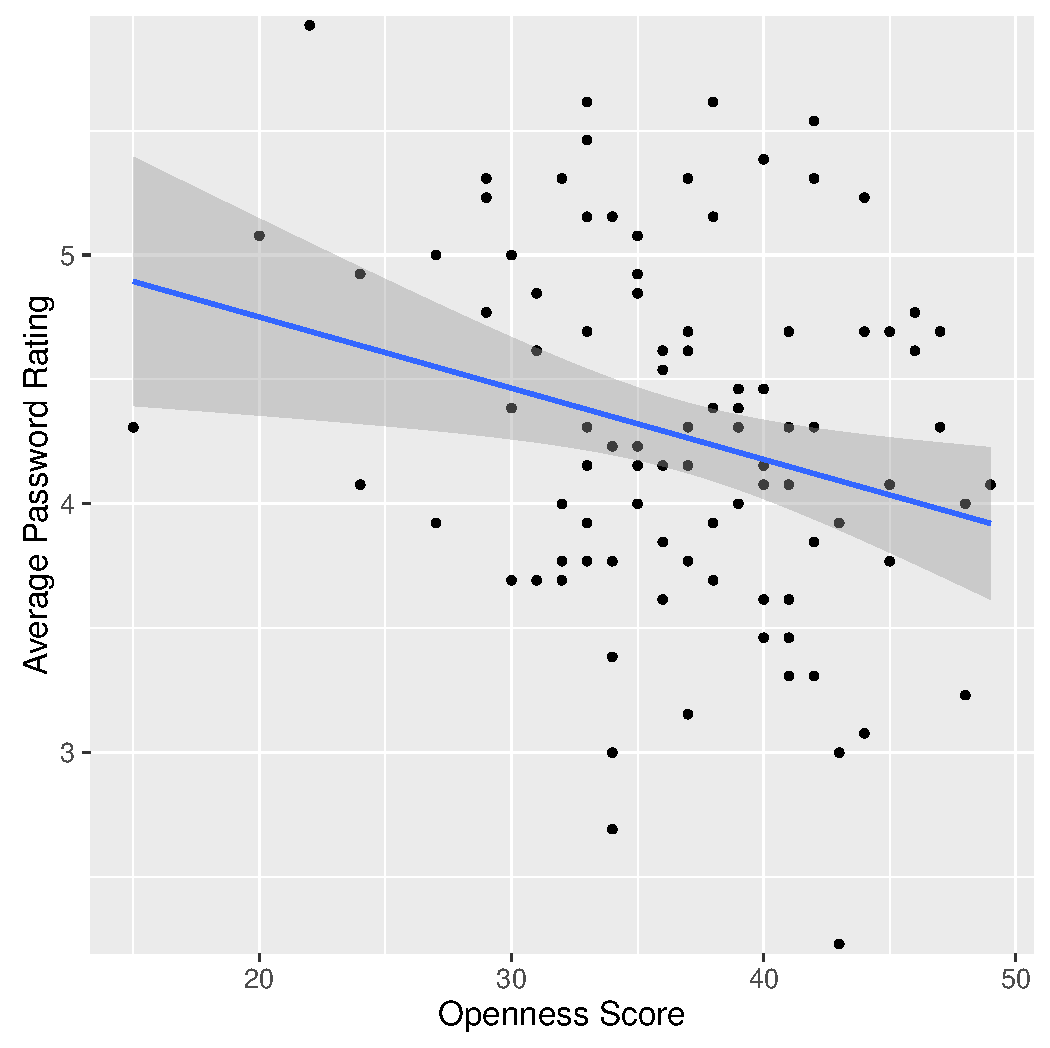
\includegraphics[width=\linewidth]{figures/Openness-ScatterPlot3}
	\caption{\label{fig:openness-scatterplot} Scatter plot of openness scores on x-axis and overall password ratings on y-axis, with fitted regression line and 95\% confidence interval. Participants scoring high on openness are a little more pessimistic in rating the strength of passwords.}
\end{figure}

%%%%%%%%%%%%%%%%%%%%%%%%%%
%%% 
%%% 		STRENGTH COMPARISON
%%% 
%%%%%%%%%%%%%%%%%%%%%%%%%%
\subsubsection{Comparisons Between Two Passwords}
We explored whether personality traits or decision making style influence how participants compare two given passwords. The regression model for the corresponding analysis is shown in Table \ref{tab:Comparison-Regression}. Here, we can see that conscientiousness was retained as predictor in all models. The most interesting association was found when one of the two passwords contained digits: With a rising number of digits, the conscientious participants favored these passwords ($\beta = 0.47, p < 0.01$), but they did not take length into account as often ($\beta = -0.12, ns$). The opposite is true for participants scoring high on the openness scale. They are more likely to vote for the longer password ($\beta = 0.27, p < 0.05$) than for the one containing digits ($\beta = -0.23, p < 0.05$). 

We also see moderate associations between decision making style and the evaluation based on length and strength as measured by zxcvbn. There is a noteworthy finding concerning people ranking high on rational or intuitive decision making style. We find that rational decision makers were worse at identifying the stronger password ($\beta = -0.35, p < 0.01$) than the intuitive decision makers ($\beta = -0.18, ns$).  

We found weak associations between the control variables and password strength assessment, mostly originating from gender or computer-science background. In the comparison task, male participants were more likely to prefer the password consisting of more character classes ($\beta = 0.21, p < 0.05$). 

In all the models, the predictive power was moderate, with an average $R^2_{adj}$ value of $0.13~(SD=0.04)$. However, the model fit was much better than before, when passwords had to be rated without a point of reference. We see that for the comparison, openness was again an important predictor, but conscientiousness was even more important. The associations between GDMS and password comparisons form a diverse spectrum with no evident pattern. 

%regression comparison

% Table generated by Excel2LaTeX from sheet 'Latex Separate Regressions'
\begin{table*}[h]
 \centering
 \small
  \caption{Regression analysis of the comparison task. Conscientiousness and openness are the most important predictors. Open participants were more likely to vote for the longer password instead of the one with digits, while the inverse is true for conscientious participants. Rational decision makers failed to identify the stronger password more often.}
             \begin{tabular}{rl|rr|rrrr}
      & Predictor & \multicolumn{1}{l}{Length} & \multicolumn{1}{l|}{Strength} & \multicolumn{1}{l}{Symbols} & \multicolumn{1}{l}{Digits} & \multicolumn{1}{l}{Cases} & \multicolumn{1}{l}{Classes} \\
\cmidrule{3-8}    \rowcolor[rgb]{ .718,  .871,  .91} \multicolumn{1}{l}{Big Five} & Neuroticism & \cellcolor[rgb]{ 1,  1,  1}  & \cellcolor[rgb]{ .98,  .627,  .459} -0.15 & \cellcolor[rgb]{ 1,  1,  1}  & \cellcolor[rgb]{ .878,  .89,  .514} 0.19 & \cellcolor[rgb]{ 1,  1,  1}  & \cellcolor[rgb]{ 1,  1,  1}  \\
    \rowcolor[rgb]{ .718,  .871,  .91}   & Extraversion & \cellcolor[rgb]{ 1,  1,  1}  & \cellcolor[rgb]{ .98,  .596,  .455} -0.18 & \cellcolor[rgb]{ 1,  1,  1}  & \cellcolor[rgb]{ 1,  1,  1}  & \cellcolor[rgb]{ 1,  1,  1}  & \cellcolor[rgb]{ 1,  1,  1}  \\
    \rowcolor[rgb]{ .718,  .871,  .91}   & Openness & \cellcolor[rgb]{ .741,  .847,  .506} \textbf{0.27} & \cellcolor[rgb]{ .914,  .898,  .514} 0.17 & \cellcolor[rgb]{ 1,  1,  1}  & \cellcolor[rgb]{ .976,  .541,  .443} \textbf{-0.23} & \cellcolor[rgb]{ 1,  1,  1}  & \cellcolor[rgb]{ .984,  .671,  .467} -0.11 \\
    \rowcolor[rgb]{ .718,  .871,  .91}   & Agreeableness & \cellcolor[rgb]{ .969,  .914,  .518} 0.14 & \cellcolor[rgb]{ .996,  .91,  .514} 0.11 & \cellcolor[rgb]{ 1,  1,  1}  & \cellcolor[rgb]{ 1,  1,  1}  & \cellcolor[rgb]{ 1,  1,  1}  & \cellcolor[rgb]{ 1,  1,  1}  \\
    \rowcolor[rgb]{ .718,  .871,  .91}   & Conscientiousness & \cellcolor[rgb]{ .984,  .659,  .467} -0.12 & \cellcolor[rgb]{ .898,  .894,  .514} 0.18 & \cellcolor[rgb]{ .969,  .914,  .518} 0.14 & \cellcolor[rgb]{ .388,  .745,  .482} \textbf{0.47} & \cellcolor[rgb]{ .878,  .89,  .514} 0.19 & \cellcolor[rgb]{ .635,  .816,  .498} \textbf{0.33} \\
    \rowcolor[rgb]{ .988,  .835,  .706} \multicolumn{1}{l}{GDMS} & Rational & \cellcolor[rgb]{ .976,  .486,  .431} \textbf{-0.28} & \cellcolor[rgb]{ .973,  .412,  .42} \textbf{-0.35} & \cellcolor[rgb]{ 1,  1,  1}  & \cellcolor[rgb]{ .898,  .894,  .514} 0.18 & \cellcolor[rgb]{ 1,  1,  1}  & \cellcolor[rgb]{ 1,  1,  1}  \\
    \rowcolor[rgb]{ .988,  .835,  .706}   & Intuitive & \cellcolor[rgb]{ .98,  .627,  .459} -0.15 & \cellcolor[rgb]{ .98,  .596,  .455} -0.18 & \cellcolor[rgb]{ 1,  1,  1}  & \cellcolor[rgb]{ 1,  1,  1}  & \cellcolor[rgb]{ 1,  1,  1}  & \cellcolor[rgb]{ 1,  1,  1}  \\
    \rowcolor[rgb]{ .988,  .835,  .706}   & Dependent & \cellcolor[rgb]{ 1,  1,  1}  & \cellcolor[rgb]{ 1,  1,  1}  & \cellcolor[rgb]{ 1,  1,  1}  & \cellcolor[rgb]{ 1,  1,  1}  & \cellcolor[rgb]{ .984,  .918,  .518} 0.13 & \cellcolor[rgb]{ 1,  1,  1}  \\
    \rowcolor[rgb]{ .988,  .835,  .706}   & Avoidant & \cellcolor[rgb]{ 1,  1,  1}  & \cellcolor[rgb]{ 1,  1,  1}  & \cellcolor[rgb]{ .984,  .659,  .467} -0.12 & \cellcolor[rgb]{ .827,  .875,  .51} 0.22 & \cellcolor[rgb]{ 1,  1,  1}  & \cellcolor[rgb]{ 1,  1,  1}  \\
    \rowcolor[rgb]{ .988,  .835,  .706}   & Spontaneous & \cellcolor[rgb]{ 1,  1,  1}  & \cellcolor[rgb]{ 1,  1,  1}  & \cellcolor[rgb]{ 1,  1,  1}  & \cellcolor[rgb]{ 1,  1,  1}  & \cellcolor[rgb]{ .98,  .616,  .459} -0.16 & \cellcolor[rgb]{ 1,  1,  1}  \\
      & Education &   &   &   & \cellcolor[rgb]{ .984,  .659,  .467} -0.12 &   &  \\
      & CS Background & \cellcolor[rgb]{ .843,  .878,  .51} \textbf{0.21} & \cellcolor[rgb]{ .843,  .878,  .51} \textbf{0.21} &   & \cellcolor[rgb]{ .984,  .682,  .471} -0.1 &   &  \\
      & Male &   &   & \cellcolor[rgb]{ .843,  .878,  .51} \textbf{0.21} & \cellcolor[rgb]{ .949,  .91,  .518} 0.15 & \cellcolor[rgb]{ .706,  .839,  .502} \textbf{0.29} & \cellcolor[rgb]{ .843,  .878,  .51} \textbf{0.21} \\
    \midrule
      & F & 3.95 & 3.78 & 3.37 & 3.13 & 3.86 & 5.75 \\
      & df & 6 & 8 & 3 & 8 & 4 & 3 \\
      & p & \multicolumn{1}{l}{< 0.01} & \multicolumn{1}{l|}{< 0.01} & \multicolumn{1}{l}{< 0.05} & \multicolumn{1}{l}{< 0.01} & \multicolumn{1}{l}{< 0.01} & \multicolumn{1}{l}{<0.01} \\
      & R$^2$ & \cellcolor[rgb]{ .533,  .804,  .608} 0.2 & \cellcolor[rgb]{ .388,  .745,  .482} 0.25 & \cellcolor[rgb]{ .82,  .922,  .855} 0.1 & \cellcolor[rgb]{ .506,  .792,  .584} 0.21 & \cellcolor[rgb]{ .706,  .875,  .757} 0.14 & \cellcolor[rgb]{ .675,  .863,  .729} 0.15 \\
      & Adjusted R$^2$& \cellcolor[rgb]{ .494,  .788,  .576} 0.15 & \cellcolor[rgb]{ .388,  .745,  .482} 0.18 & \cellcolor[rgb]{ .776,  .906,  .82} 0.07 & \cellcolor[rgb]{ .494,  .788,  .576} 0.15 & \cellcolor[rgb]{ .671,  .863,  .729} 0.1 & \cellcolor[rgb]{ .565,  .82,  .635} 0.13 \\
    \bottomrule
    \bottomrule
    \end{tabular}%
  \label{tab:Comparison-Regression}%
\end{table*}%


\subsubsection{Qualitative Findings}
While entering an elaborate response was not mandatory, all but one participant (\textit{n}=99) gave a brief and in most cases comprehensible explanation for their ratings. The numbers do not necessarily add up to \textit{n}, because answers could receive multiple codes.

We identified four overall themes in how the participants approached rating passwords: \textit{Character diversity}, \textit{creation strategy}, \textit{predictability} and \textit{other}. The character diversity code consists of participants mentioning the importance of symbols (69), digits (52), upper-/lowercase letters (45) and general variety of characters (16). Regarding the creation strategy, many participants penalized passwords when they contained actual words (40) or personal information (3). The predictability category was divided into answers referring to character substitutions (10), patterns (17), guessability (12), randomness (20), length (25) and the position of symbols/digits (6). The other themes were established from 8 participants using technical jargon (e.g. ``attack'' or ``brute force'') and those who identified the obfuscated passwords (2). 

\subsubsection{Synthesis}
We found that participants evaluate password strength by looking for specific patterns. Regression models and qualitative analysis show that respondents mostly penalized lack of diversity and randomness which is consistent with the related work \cite{Ur2016PerceptionsPassword}. Thus, the associations originating from different personality types or decision making style were small in many cases, but not negligible. The education level was generally insignificant regarding the strength evaluation. However, technical background and gender played a role in the comparison task, because male participants were more likely influenced by character variety. The predictive power of the independent variables was higher in the comparison task than in the standalone rating. The most important factors were \textbf{openness} on \textbf{conscientiousness} from the Big-Five model, and \textbf{rationality} from the GDMS. 

%%%%%%%%%%%%%%%%%%%%%%%%%%%%%%%%%%%%%%%%%%%
%%%%
%%%%
%%%%			STUDY  3 THREE DREI
%%%%			SELECTION
%%%%
%%%%
%%%%%%%%%%%%%%%%%%%%%%%%%%%%%%%%%%%%%%%%%%%
\section{Study 3: Password Selection}
% ALINE
% GOALS
As a final step in our ``password personality'' exploration, we ran an online survey. Having investigated preferences for policies and the perception of passwords, the main goal of the third study was to evaluate potential associations between personality and password \textit{selection}. To overcome some of the limitations of the previous study, we hoped to increase the sample size and reduce the number of items during the study. Moreover, further answers about the participants' explanations and motivations were considered to better understand the weight of personality factors. We determined the following research questions: 1) Are there correlations between password features (topology) and personality traits? 2) Do certain facets of personality shine through in password management behavior, e.g. the tendency to write down passwords?

\subsection{Procedure and Tools}
The study was designed to take no more than ten minutes. The briefing page informed participants about the purpose of the study and data disclosure policies. After acknowledging the conditions of participation, respondents were asked to create a password. To boost ecological validity, we provided a fictitious but realistic scenario \cite{Komanduri2011OfPasswordsAndPeople}. The task was to come up with a new password for a new email account that they were going to use as their main address. Further, the instruction pointed out that the incentive would only be paid of if the participants chose a password they could recall later on. A \textit{basic8} policy was enforced, as it is one of the most representative policies in the wild (see chapter \ref{chap:policies_reuse}). This loose policy would also allow for both very complex and rather simple passwords, which could be associated with personality traits. Having successfully confirmed the password, respondents were taken to a questionnaire about demographics, just like in the first two studies. 

Next, participants completed the BFI-K questionnaire consisting of 21 items that have to be rated on a 5-point scale. We opted not to use the 50-item inventory for the sake of saving time. We added an item that served as an attention check. It asked to respond to this item with ``disagree''. Failure to follow this instruction allowed us to drop the response from the dataset. The resulting 22 items were shuffled to avoid sequence effects. 

Afterwards, we surveyed respondents about their password management behaviors and preferences. We used multiple-choice and open responses to collect qualitative, self-reported data. For instance, we wanted to know how they cope with multiple accounts or how they reuse passwords. The survey concluded with a recall task, where participants provided their initially chosen password. They could try as often as they liked, and the number of attempts were recorded. In case they were unable to recall their password, they could proceed anyhow and take part in the lottery. If they chose to provide an email address in the final step, this data was stored separately from the questionnaire data to avoid privacy issues. 

\subsection{Recruitment and Sample}
Participants were invited via a university newsletter, and snowballing the link via personal connections and posts on social networks. The questionnaire was in German and participants were screened about their command of the German language. We instructed participants to take the survey on a desktop. 
%TODO aline says 184 but the data set is smaller :-/ ?
%all the following numbers are from the smaller data set.
184 people completed the survey, but we had to drop the responses of 8 participants because their reponse timings were too unrealistic. From the 176 remaining respondents, 89 were male, 86 female and 1 preferred not to answer. 116 were students, i.e. a rather high proportion (66\%). Consequently, the average age was 25 years (range [16;55], $SD$=6, $Md$= 24). 67 (38\%) reportedly had an IT-background. 129 respondents chose to participate in the raffle for shopping vouchers. 

\subsection{Limitations}
\todo{Password selection not realistic / attention check item was badly placed and not well explained. 30 feedback emails.}

\subsection{Results}
% descriptives
The resulting passwords had a median-length of 10 characters ([8;22]), i.e. many participants went beyond the minimum requirement. Figure \ref{fig:personality:study3:metrics-overview} visualizes additional metrics that show that passwords were stronger than expected. In the following, we try to fit generalized additive models to the data using big-five trait scores as covariates. 

\begin{figure}[tbph]
	\centering
	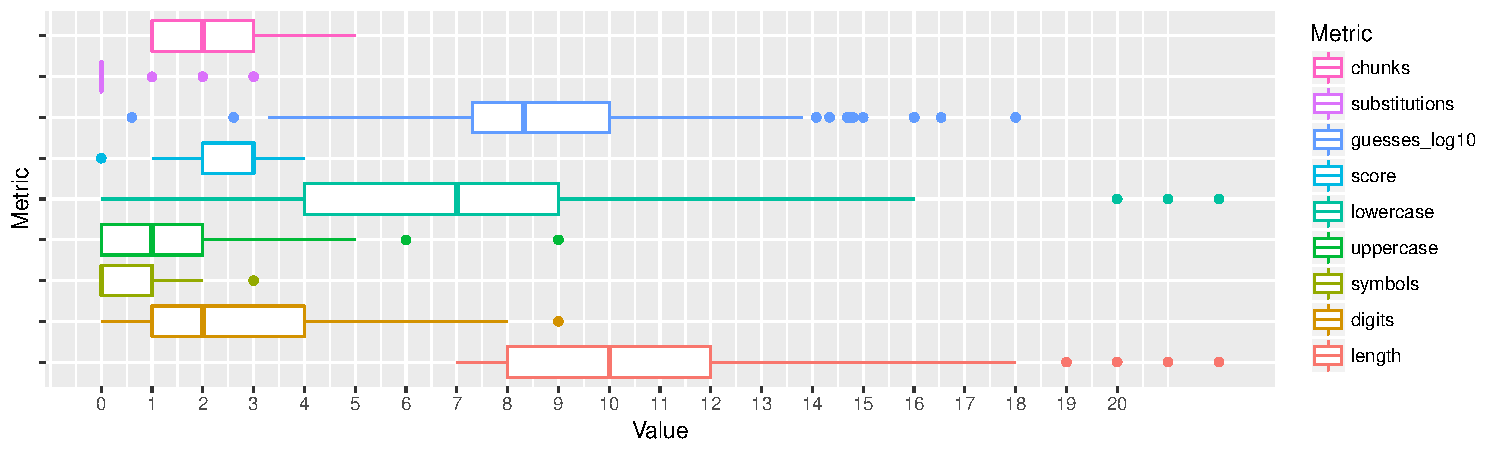
\includegraphics[width=1\linewidth]{figures/personality/study3-metrics-overview}
	\caption{\label{fig:personality:study3:metrics-overview} Zxcvbn metrics for user selected passwords.}
\end{figure}

% maximum R-sq 
\subsubsection{Password Composition}
First, we use zxcvbn metrics as response variables, i.e. we explore marginal associations from big five traits. As before, we include age, gender and IT-background as control covariates. 

\subsubsection{Memorability}


\subsection{Password Management Strategies}
% binary -- logit model ``write down'': yes no

\subsection{Learnings}


%%%%%%%%%%%%%%%%%%%%%%%%%%%%%%%%%%%%%%%%%%%
%%%%
%%%%
%%%%			GENERAL DISCUSSION
%%%%
%%%%%%%%%%%%%%%%%%%%%%%%%%%%%%%%%%%%%%%%%%%
\section{Discussion and Implications}
%In this section we interpret the results and hope to shed light on potential explanations for their origins. % and show the implications for password-authentication systems.

%TODO more elaborately discuss the origin of the results.
% Table generated by Excel2LaTeX from sheet 'Personality Overview'
\begin{table}[tbp]
  \centering
  \caption{\label{tab:personality:associations-overview}
  	Overview of significant associations between Big-Five traits, control factors, and different metrics across three studies. Arrows indicate direction of the associations, colors also highlight significance levels (red/ocher: $p$ < 0.05/0.1 negative assoc., greens: $p$ < 0.001/0.01/0.05/0.1 positive assoc.) Openness and Conscientiousness are the most important factors from the Big-Five model, and having an IT background was an indispensable control factor.
  }\resizebox{\linewidth}{!}{
    \begin{tabular}{p{6.5cm}rp{0.8cm}rrrrrrrr}
    \rowcolor[rgb]{ .38,  .612,  1} \textcolor[rgb]{ 1,  1,  1}{\textbf{Metric}} & \multicolumn{1}{l}{\textcolor[rgb]{ 1,  1,  1}{\textbf{Type}}} & \multicolumn{1}{p{0.8cm}|}{\textcolor[rgb]{ 1,  1,  1}{\textbf{Study}}} & \multicolumn{1}{c}{\textcolor[rgb]{ 1,  1,  1}{\textbf{O}}} & \multicolumn{1}{c}{\textcolor[rgb]{ 1,  1,  1}{\textbf{C}}} & \multicolumn{1}{c}{\textcolor[rgb]{ 1,  1,  1}{\textbf{E}}} & \multicolumn{1}{c}{\textcolor[rgb]{ 1,  1,  1}{\textbf{A}}} & \multicolumn{1}{c|}{\textcolor[rgb]{ 1,  1,  1}{\textbf{N}}} & \multicolumn{1}{l}{\textcolor[rgb]{ 1,  1,  1}{\textbf{Age}}} & \multicolumn{1}{l}{\textcolor[rgb]{ 1,  1,  1}{\textbf{Gender}}} & \multicolumn{1}{l}{\textcolor[rgb]{ 1,  1,  1}{\textbf{IT}}} \\
    
    Difficulty to create 2word12 PW & \multicolumn{1}{l}{Usability} & \multicolumn{1}{r|}{1} &       &       &       &       & \multicolumn{1}{r|}{} &       & \multicolumn{1}{l}{\cellcolor[rgb]{ .486,  .682,  0} \textcolor[rgb]{ 1,  1,  1}{\emoji{2197} (< .1)}} &  \\

    Difficulty to create 1emoji12 PW & \multicolumn{1}{l}{Usability} & \multicolumn{1}{r|}{1} &       &       &       & \multicolumn{1}{l}{\cellcolor[rgb]{ .871,  .549,  0} \textcolor[rgb]{ 1,  1,  1}{\emoji{2198} (< .1)}} & \multicolumn{1}{l|}{\cellcolor[rgb]{ .973,  .463,  .427} \textcolor[rgb]{ 1,  1,  1}{\emoji{2198} (< .05)}} &       & \multicolumn{1}{l}{\cellcolor[rgb]{ .486,  .682,  0} \textcolor[rgb]{ 1,  1,  1}{\emoji{2197} (< .1)}} &  \\
    
    Preference of 3class12 policy & \multicolumn{1}{l}{Attitude} & \multicolumn{1}{r|}{1} &       &       &       & \multicolumn{1}{l}{\cellcolor[rgb]{ .973,  .463,  .427} \textcolor[rgb]{ 1,  1,  1}{\emoji{2198} (< .05)}} & \multicolumn{1}{r|}{} &       &       &  \\
    
    Preference of 2word12 policy & \multicolumn{1}{l}{Attitude} & \multicolumn{1}{r|}{1} &       &       & \multicolumn{1}{l}{\cellcolor[rgb]{ .973,  .463,  .427} \textcolor[rgb]{ 1,  1,  1}{\emoji{2198} (< .05)}} &       & \multicolumn{1}{r|}{} &       &       &  \\
    
    Preference of 1emoji12 policy & \multicolumn{1}{l}{Attitude} & \multicolumn{1}{r|}{1} &       &       &       & \multicolumn{1}{l}{\cellcolor[rgb]{ 0,  .729,  .22} \textcolor[rgb]{ 1,  1,  1}{\emoji{2197} (< .05)}} & \multicolumn{1}{l|}{\cellcolor[rgb]{ .486,  .682,  0} \textcolor[rgb]{ 1,  1,  1}{\emoji{2197} (< .1)}} &       &       & \multicolumn{1}{l}{\cellcolor[rgb]{ .973,  .463,  .427} \textcolor[rgb]{ 1,  1,  1}{\emoji{2198} (< .05)}} \\
    
    Time to create PW & \multicolumn{1}{l}{Usability} & \multicolumn{1}{r|}{1} &       & \multicolumn{1}{l}{\cellcolor[rgb]{ .973,  .463,  .427} \textcolor[rgb]{ 1,  1,  1}{\emoji{2198} (< .05)}} &       &       & \multicolumn{1}{l|}{\cellcolor[rgb]{ .871,  .549,  0} \textcolor[rgb]{ 1,  1,  1}{\emoji{2198} (< .1)}} &       & \multicolumn{1}{l}{\cellcolor[rgb]{ 0,  .753,  .545} \textcolor[rgb]{ 1,  1,  1}{\emoji{2197} (< .01)}} &  \\
    \midrule
    
    Overall tendency to judge PWs & \multicolumn{1}{l}{Behavior} & \multicolumn{1}{r|}{2} & \multicolumn{1}{l}{\cellcolor[rgb]{ .973,  .463,  .427} \textcolor[rgb]{ 1,  1,  1}{\emoji{2198} (< .05)}} &       &       &       & \multicolumn{1}{r|}{} &       &       &  \\
    
    Comparing PWs based on complexity & \multicolumn{1}{l}{Behavior} & \multicolumn{1}{r|}{2} &       & \multicolumn{1}{l}{\cellcolor[rgb]{ 0,  .753,  .545} \textcolor[rgb]{ 1,  1,  1}{\emoji{2197} (< .01)}} &       &       & \multicolumn{1}{r|}{} &       & \multicolumn{1}{l}{\cellcolor[rgb]{ .973,  .463,  .427} \textcolor[rgb]{ 1,  1,  1}{\emoji{2198} (< .05)}} &  \\
    
    Comparing PWs based on digits & \multicolumn{1}{l}{Behavior} & \multicolumn{1}{r|}{2} & \multicolumn{1}{l}{\cellcolor[rgb]{ .973,  .463,  .427} \textcolor[rgb]{ 1,  1,  1}{\emoji{2198} (< .05)}} & \multicolumn{1}{l}{\cellcolor[rgb]{ 0,  .749,  .769} \textcolor[rgb]{ 1,  1,  1}{\emoji{2197} (< .001)}} &       &       & \multicolumn{1}{r|}{} &       &       &  \\
    
    Comparing PWs based on uppercase & \multicolumn{1}{l}{Behavior} & \multicolumn{1}{r|}{2} &       & \multicolumn{1}{l}{\cellcolor[rgb]{ .486,  .682,  0} \textcolor[rgb]{ 1,  1,  1}{\emoji{2197} (< .1)}} &       &       & \multicolumn{1}{r|}{} & \multicolumn{1}{l}{\cellcolor[rgb]{ .871,  .549,  0} \textcolor[rgb]{ 1,  1,  1}{\emoji{2198} (< .1)}} &       &  \\
    
    Comparing PWs based on length & \multicolumn{1}{l}{Behavior} & \multicolumn{1}{r|}{2} & \multicolumn{1}{l}{\cellcolor[rgb]{ 0,  .729,  .22} \textcolor[rgb]{ 1,  1,  1}{\emoji{2197} (< .05)}} & \multicolumn{1}{l}{\cellcolor[rgb]{ .973,  .463,  .427} \textcolor[rgb]{ 1,  1,  1}{\emoji{2198} (< .05)}} &       &       & \multicolumn{1}{r|}{} & \multicolumn{1}{l}{ } &       & \multicolumn{1}{l}{\cellcolor[rgb]{ 0,  .729,  .22} \textcolor[rgb]{ 1,  1,  1}{\emoji{2197} (< .05)}} \\
    \midrule
    
    Length of created PW & \multicolumn{1}{l}{Behavior} & \multicolumn{1}{r|}{3} &       &       &       &       & \multicolumn{1}{l|}{\cellcolor[rgb]{ 0,  .729,  .22} \textcolor[rgb]{ 1,  1,  1}{\emoji{2197} (< .05)}} &       &       & \multicolumn{1}{l}{\cellcolor[rgb]{ 0,  .729,  .22} \textcolor[rgb]{ 1,  1,  1}{\emoji{2197} (< .05)}} \\
    
    Guess number of created PW & \multicolumn{1}{l}{Behavior} & \multicolumn{1}{r|}{3} &       &       &       &       & \multicolumn{1}{r|}{} &       &       & \multicolumn{1}{l}{\cellcolor[rgb]{ 0,  .729,  .22} \textcolor[rgb]{ 1,  1,  1}{\emoji{2197} (< .05)}} \\
    
    zxcvbn score of created PW & \multicolumn{1}{l}{Behavior} & \multicolumn{1}{r|}{3} &       &       &       &       & \multicolumn{1}{l|}{\cellcolor[rgb]{ .486,  .682,  0} \textcolor[rgb]{ 1,  1,  1}{\emoji{2197} (< .1)}} &       &       & \multicolumn{1}{l}{\cellcolor[rgb]{ 0,  .729,  .22} \textcolor[rgb]{ 1,  1,  1}{\emoji{2197} (< .05)}} \\
    
    Created PW is passphrase & \multicolumn{1}{l}{Behavior} & \multicolumn{1}{r|}{3} &       &       &       &       & \multicolumn{1}{r|}{} &       &       & \multicolumn{1}{l}{\cellcolor[rgb]{ 0,  .729,  .22} \textcolor[rgb]{ 1,  1,  1}{\emoji{2197} (< .05)}} \\
    
    Created PW is random & \multicolumn{1}{l}{Behavior} & \multicolumn{1}{r|}{3} &       &       &       &       & \multicolumn{1}{r|}{} &       & \multicolumn{1}{l}{\cellcolor[rgb]{ .973,  .463,  .427} \textcolor[rgb]{ 1,  1,  1}{\emoji{2198} (< .05)}} & \multicolumn{1}{l}{\cellcolor[rgb]{ .871,  .549,  0} \textcolor[rgb]{ 1,  1,  1}{\emoji{2198} (< .1)}} \\
    
    Cope by memorizing PW & \multicolumn{1}{l}{Behavior} & \multicolumn{1}{r|}{3} &       & \multicolumn{1}{l}{\cellcolor[rgb]{ .871,  .549,  0} \textcolor[rgb]{ 1,  1,  1}{\emoji{2198} (< .1)}} & \multicolumn{1}{l}{\cellcolor[rgb]{ 0,  .729,  .22} \textcolor[rgb]{ 1,  1,  1}{\emoji{2197} (< .05)}} & \multicolumn{1}{l}{\cellcolor[rgb]{ .871,  .549,  0} \textcolor[rgb]{ 1,  1,  1}{\emoji{2198} (< .1)}} & \multicolumn{1}{r|}{} & \multicolumn{1}{l}{\cellcolor[rgb]{ .871,  .549,  0} \textcolor[rgb]{ 1,  1,  1}{\emoji{2198} (< .1)}} &       & \multicolumn{1}{l}{\cellcolor[rgb]{ .973,  .463,  .427} \textcolor[rgb]{ 1,  1,  1}{\emoji{2198} (< .05)}} \\
    
    Cope by reusing PW & \multicolumn{1}{l}{Behavior} & \multicolumn{1}{r|}{3} &       &       &       & \multicolumn{1}{l}{\cellcolor[rgb]{ .871,  .549,  0} \textcolor[rgb]{ 1,  1,  1}{\emoji{2198} (< .1)}} & \multicolumn{1}{r|}{} &       &       & \multicolumn{1}{l}{\cellcolor[rgb]{ .973,  .463,  .427} \textcolor[rgb]{ 1,  1,  1}{\emoji{2198} (< .05)}} \\
    
    Cope by using PWM & \multicolumn{1}{l}{Behavior} & \multicolumn{1}{r|}{3} & \multicolumn{1}{l}{\cellcolor[rgb]{ .973,  .463,  .427} \textcolor[rgb]{ 1,  1,  1}{\emoji{2198} (< .05)}} &       &       &       & \multicolumn{1}{r|}{} &       & \multicolumn{1}{l}{\cellcolor[rgb]{ .871,  .549,  0} \textcolor[rgb]{ 1,  1,  1}{\emoji{2198} (< .1)}} & \multicolumn{1}{l}{\cellcolor[rgb]{ 0,  .729,  .22} \textcolor[rgb]{ 1,  1,  1}{\emoji{2197} (< .05)}} \\
    
    Cope by using paper / files & \multicolumn{1}{l}{Behavior} & \multicolumn{1}{r|}{3} &       &       & \multicolumn{1}{l}{\cellcolor[rgb]{ .973,  .463,  .427} \textcolor[rgb]{ 1,  1,  1}{\emoji{2198} (< .05)}} &       & \multicolumn{1}{r|}{} &       &       &  \\
    \midrule
    \midrule
    %\textbf{Number of significant associations (p < 0.05)} &       &       & \textbf{4} & \textbf{4} & \textbf{3} & \textbf{2} & \textbf{2} & \textbf{0} & \textbf{2} & \textbf{8} \\
    \multicolumn{3}{l}{\textbf{Number of significant associations (p < 0.05 [0.1] )}} & \textbf{4~[4]} & \textbf{4~[6]} & \textbf{3~[3]} & \textbf{2~[5]} & \textbf{2~[5]} & \textbf{0~[2]} & \textbf{3~[6]} & \textbf{9~[9]} \\
    \end{tabular}%
}
\end{table}%
%tab:personality:associations-overview

% Egelman says:
\subsection{Overarching Themes and User Segments}
Egelman and Peer highlighted the importance of the the question \textit{which psychographic segments should be targeted [in security and privacy mitigations]?} While they focused on their newly developed SeBIS scale and other psychometric constructs, we are able to give new pointers for segmenting users based on their Big-Five traits in conjunction with demographic factors. To approach the segmentation, we can look at the overall influences of personality and demographic factors on different metrics. Table \ref{tab:personality:associations-overview} lists all significant marginal associations from all three studies. 

% Neuroticism
\paragraph{Neuroticism} In study 1, the primary observation was that neuroticism was associated with difficulty to create an emoji password. Neuroticism was not associated with any perception metric in study 2, but the third study revealed an interesting association between neuroticsm and self-selected passwords. Metrics in the first and third study revolve around password \textit{creation}: It appears to be both \textbf{easier} to find a password expressing emotions for participants scoring high on neuroticism, and their passwords turned out significantly \textbf{longer} in the third study. 
% story: ``I see the benefit of creating stronger passwords, and I don't mind adding something I like to memorize them, so emojis inside passwords might be cool.''
Thus, targeting neuroticism with persuasive interventions during password creation might boost these positive associations. Nudges should thus focus on making emotional state more \textit{salient} and point out benefits of password length to \textit{positively reinforce} this behavior. 

% Openness
\paragraph{Openness} The usability of different composition policies was not associated with openness, but the perception of password strength showed conclusive associations in that passwords were generally judged \textbf{weaker} with higher openness scores. Participants strongly showing the openness trait were also more likely to base their decision on \textbf{password length} rather than the number of digits. In study 3, we observed that coping strategies involving a password manager were \textbf{less likely} to be found with participants with high openness scores. 
% paraphrased story: ``your passwords are weak, mine are stronger, because they are longer and I don't need help remembering them!''
The significant associations, and absence thereof, tell a conclusive story if we look at passphrases and mnemonic phrase-based passwords. Those types of passwords are strong and often not overly complex \cite{Keith2009PassphraseDesign,Kuo2006HumanSelectionMnemonic,Shay2012CorrectHorseBatteryStaple}. Passphrases, for instance, are a technique to facilitate memorization. They also easily exceed length requirements. If they consist of uppercase and lowercase letters, and are separated with regular punctuation symbols, there is no need to add digits to meet a three-class requirement: the passphrase is already complex enough. All this is visible in the study behavior of participants scoring high on openness, despite the absence of associations between openness and the type of created password in study 3. 

% Conscientiousness
\paragraph{Conscientiousness} Like openness, conscientiousness was a major factor in study 2. There was evidence that participants, who strongly show this trait, tend to believe a more \textbf{complex} password is better than a long password. We could explain this finding by looking at the attributes that are usually found with conscientious people: diligence and neatness. Following password rules requires these facets to ensure a strong outcome. The results in study 1 (less time taken to create a password) and study 3 (slight tendency to refrain from memorizing passwords) are harder to interpret. It is expectable that crafting a strong memorable password takes due diligence and more time, thus the shorter time spent by conscientious participants is counterintuitive. Perhaps it is due to the measurement approach in our study. We started taking the time as soon as the password field was focused and the timing ended when the field lost focus (``blur'' event). It is possible that conscientious participants took their time to reflect on what they wanted to enter into the field, and only then started the task. However, we do not have the data to support this argument.
% story: ``I think a strong password needs to have digits and symbols, then it can be shorter. Dictionary words should not be used.''


% Agreeableness and Extraversion
\paragraph{Agreeableness and Extraversion} Table \ref{tab:personality:associations-overview} shows that agreeableness only showed a conclusive result in study 1. A more demanding policy like 3class12 did not appeal to participants scoring high on agreeableness, while they did favor the emoji-policy much more. Cheerfulness, empathy and cooperation are often characteristics represented by this trait. 
% story: ``hey that's cool, let me see which emoji I can choose to come up with something memorable that matches the constraints and context.'' 
Participants might have favored cheerful emojis to cooperate on finding a suitable solution together. Thus, password selection could have been more fun and thus more pleasing for those participants. Since there was no sign of focusing on password strength, we hypothesize that memorability might be more important for them. 
Regarding extraversion, we found that participants scoring high on this trait disliked a word-based policy and were more likely to memorize passwords than writing them down. This is probably the most difficult result to interpret, because extraversion is a more situationally dependent trait than the four others -- a phenomenon coined as ``ambiversion'' \cite{Grant2013Ambivert}. This could have become visible if our regression models had shown more curvilinear relationships, but those were not significantly more likely for extraversion than for other traits. We therefore refrain from further discussion and note that additional data would be necessary to evaluate the stability of this predictor. 

\paragraph{Demographic Factors}
From Table \ref{tab:personality:associations-overview}, it is evident that associations with the chosen metrics are more likely to be found with demographic variables as predictors. This was especially true for study 3, where almost all outcomes were associated with having experience or education in a computer-science related field. This is an unsurprising finding, because this user group can better judge the implications of their behavior. Nevertheless, the additional factors help us segment user groups in higher detail. 

% Overall picture
\subsubsection{Deriving Segments: Password Personas}\label{sec:personality:personas}
% why do we do this / goals
With the above themes and stories, we are able to derive a number of user segments that can be targeted by security mitigations. Segmentation can inform upcoming research and design directions. For instance, segments serve the generation of hypotheses and play a role in the creation of new psychographic constructs. The ``securing'' dimension of the \gls{SeBIS} might be enriched by user archetypes to \textit{explain} attitudes and behaviors rather than just measuring them. Here, \glspl{persona} constitute a common design tool for segmentation. These fictional users can be targeted in the design of persuasive interventions. From the data of three studies on password personality, and backed up by related work, I created a set of four ``password personas'' that inform design choices in Part \ref{part:design_space} of this thesis. They are shown in Figure \ref{fig:personality:personas}. At this point, the personas still remain abstract to account for the early stage of research about password personality. Personas should be ``living'' templates that are updated based on new data \cite{Gothelf2013LeanUX}. 

\begin{figure}
	\centering
	\fcolorbox{dividergray}{white}{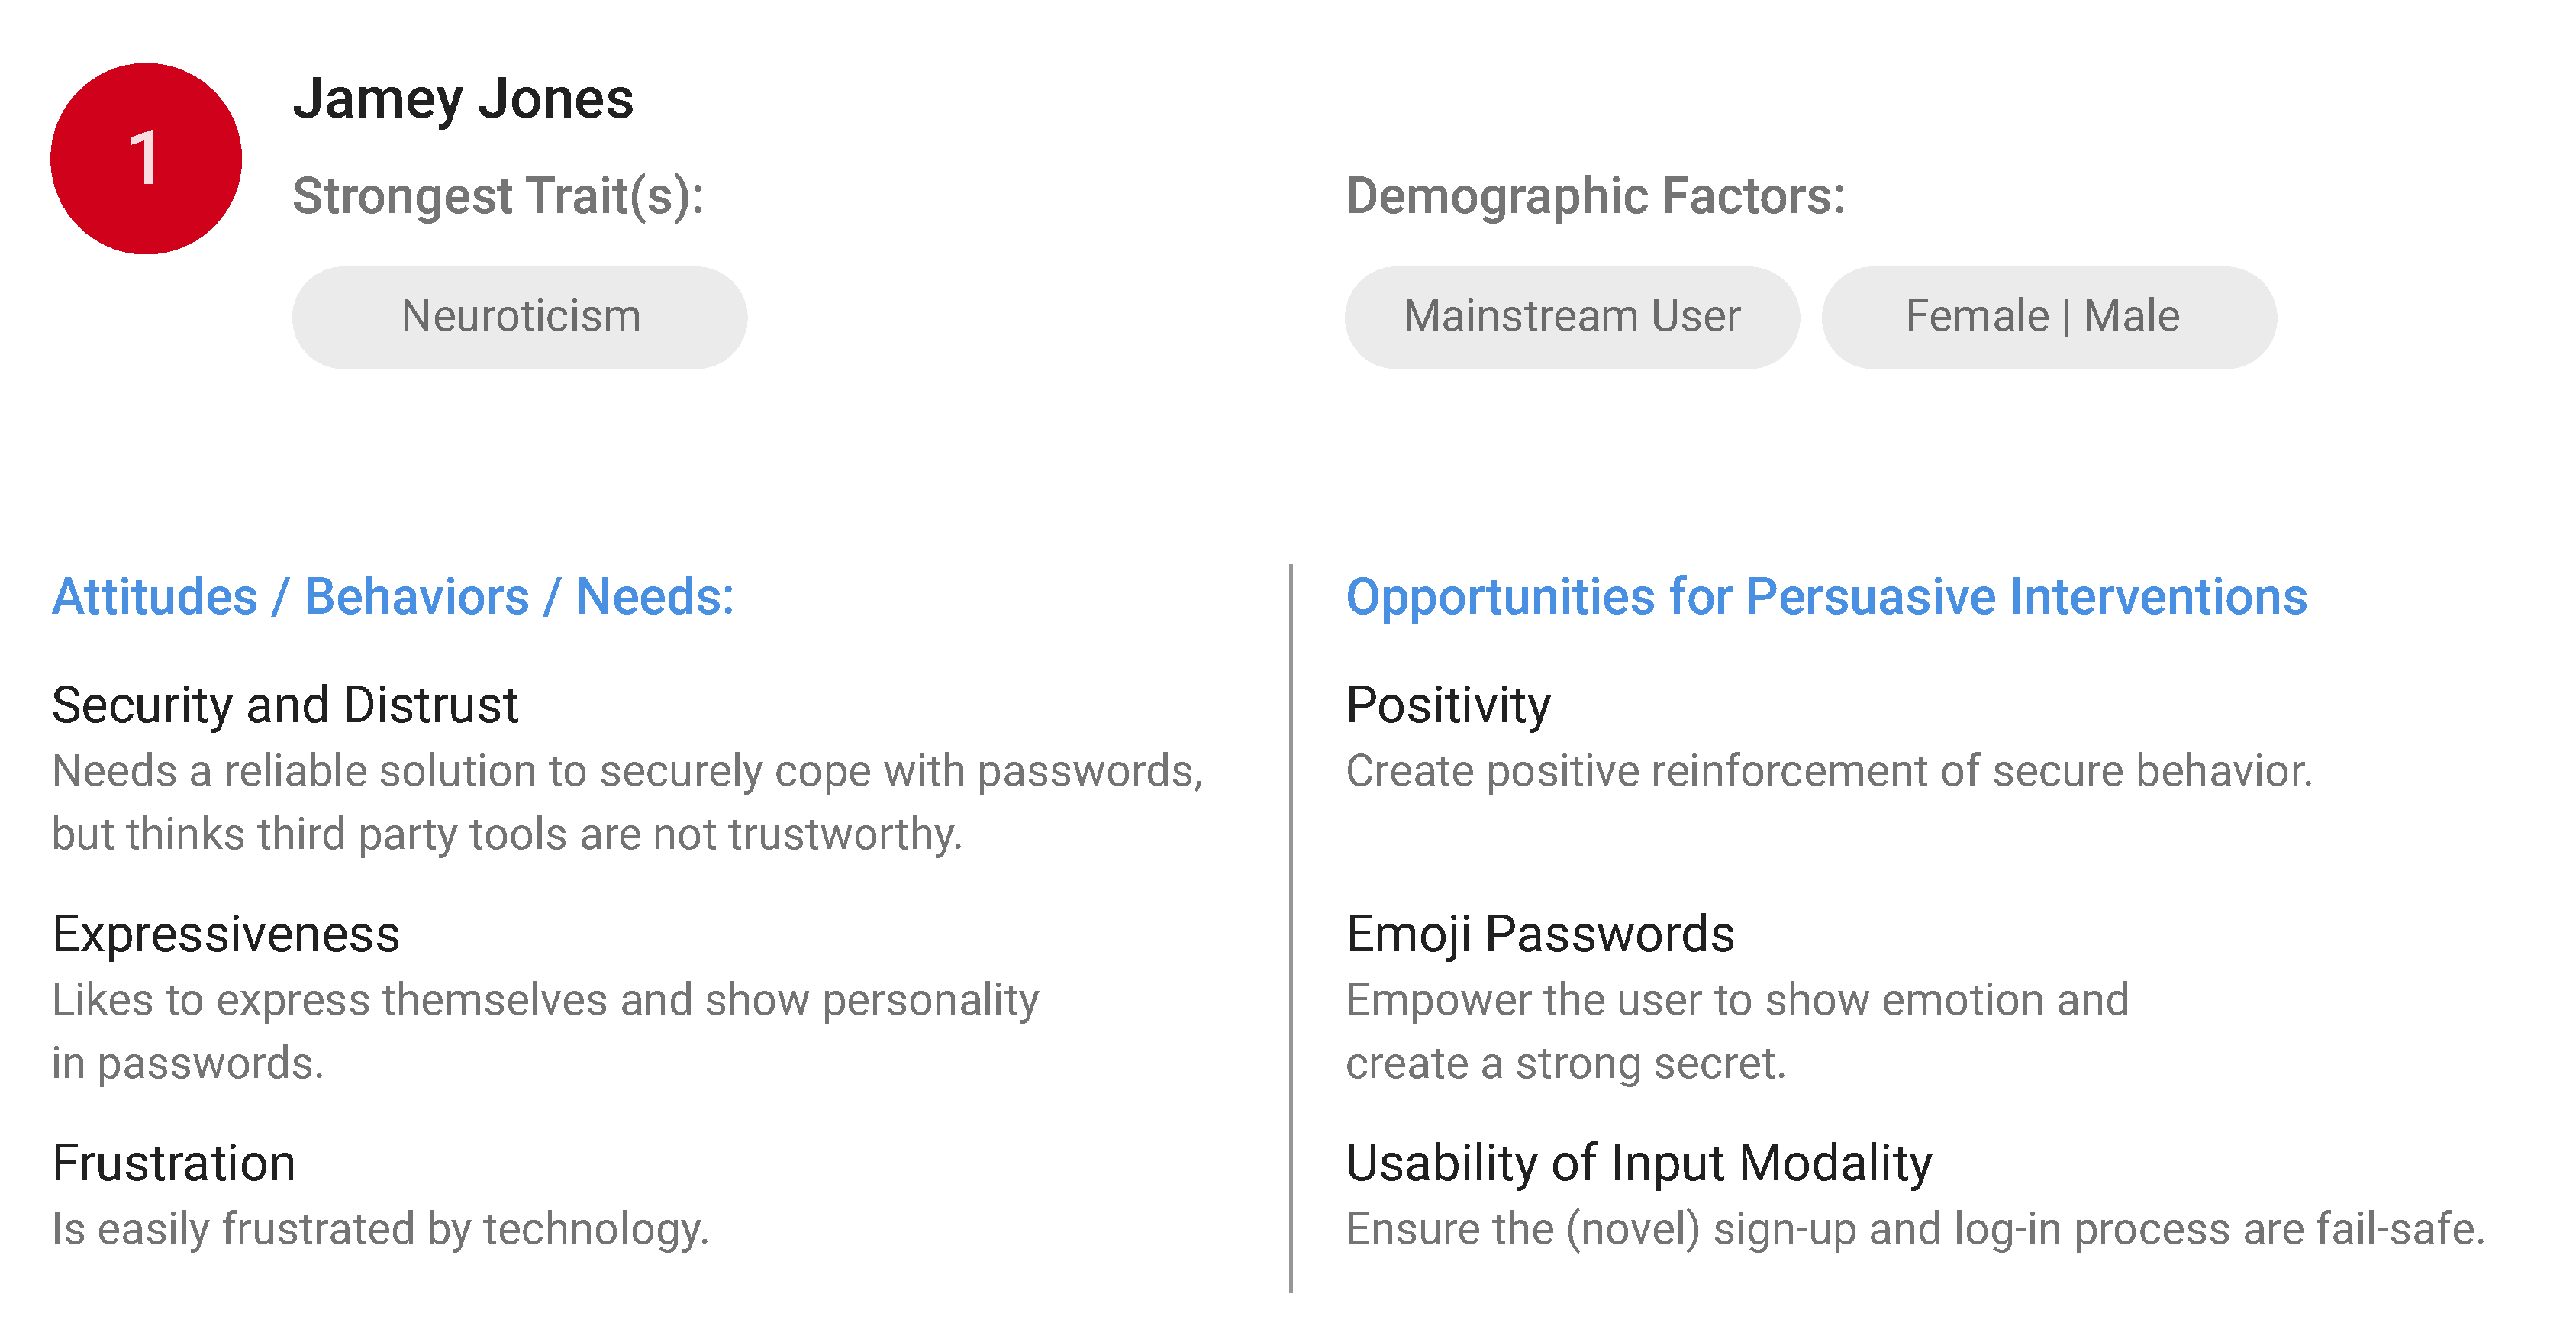
\includegraphics[width=0.7\linewidth]{personality/personas/Neurotic-Persona}}
	\fcolorbox{dividergray}{white}{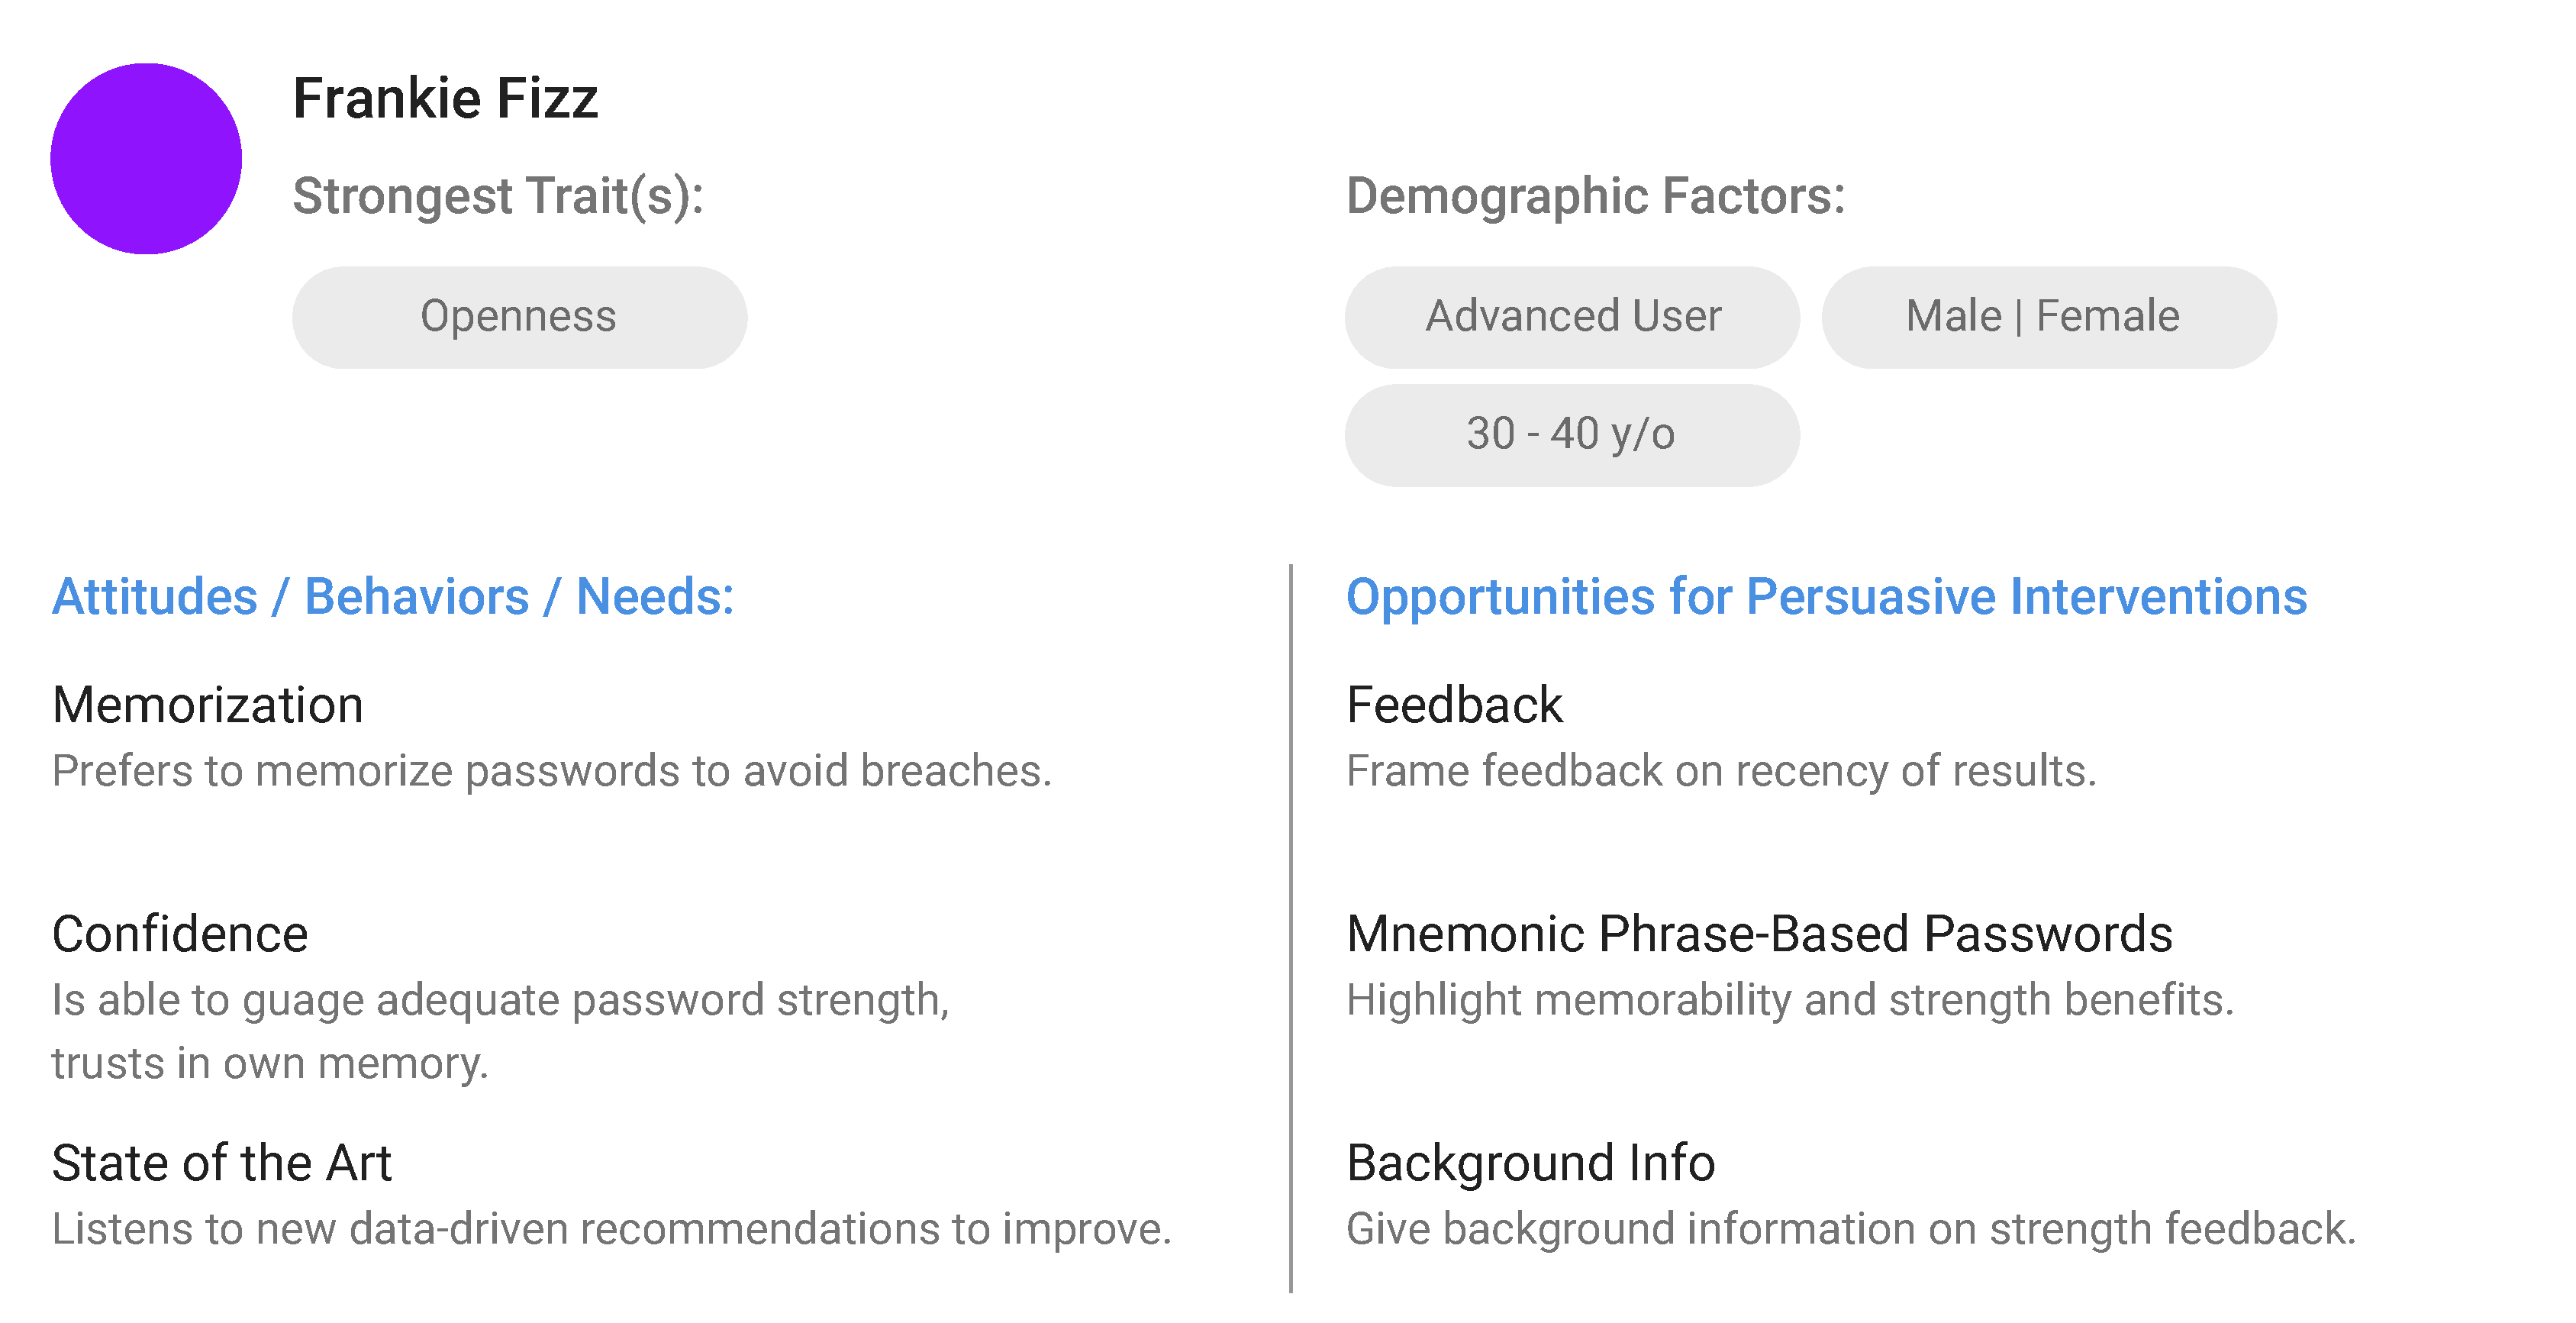
\includegraphics[width=0.7\linewidth]{personality/personas/Open-Persona}}
	\fcolorbox{dividergray}{white}{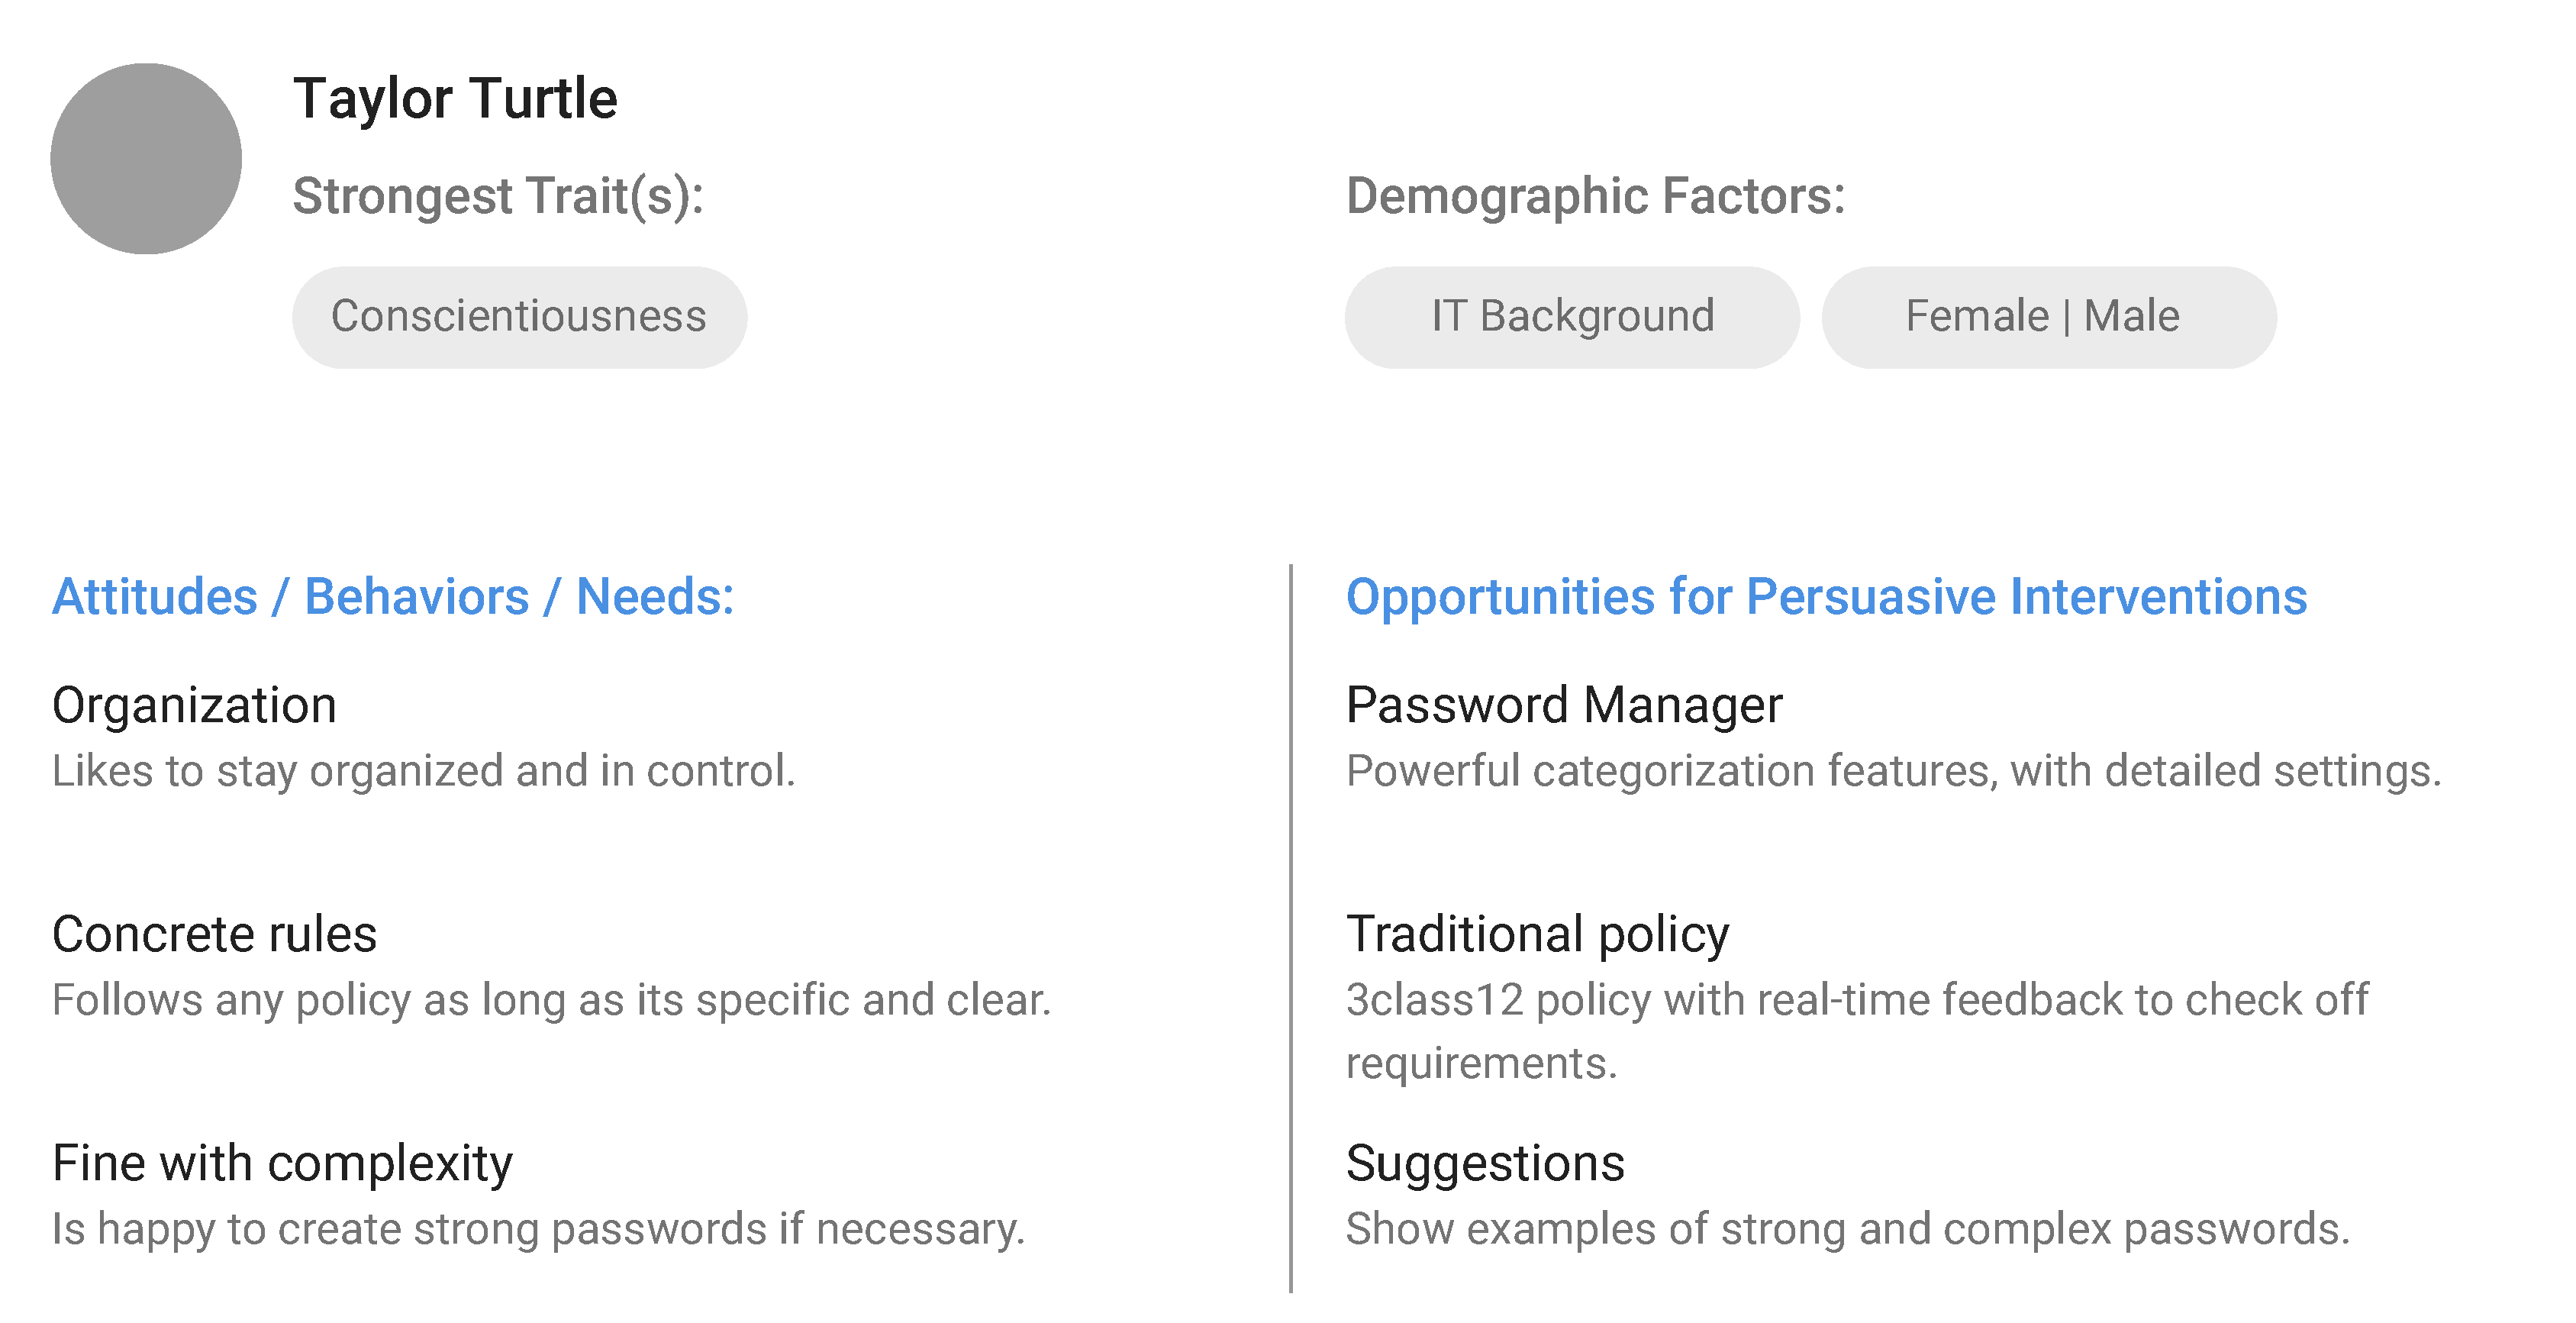
\includegraphics[width=0.7\linewidth]{personality/personas/Conscientious-Persona}}
	\fcolorbox{dividergray}{white}{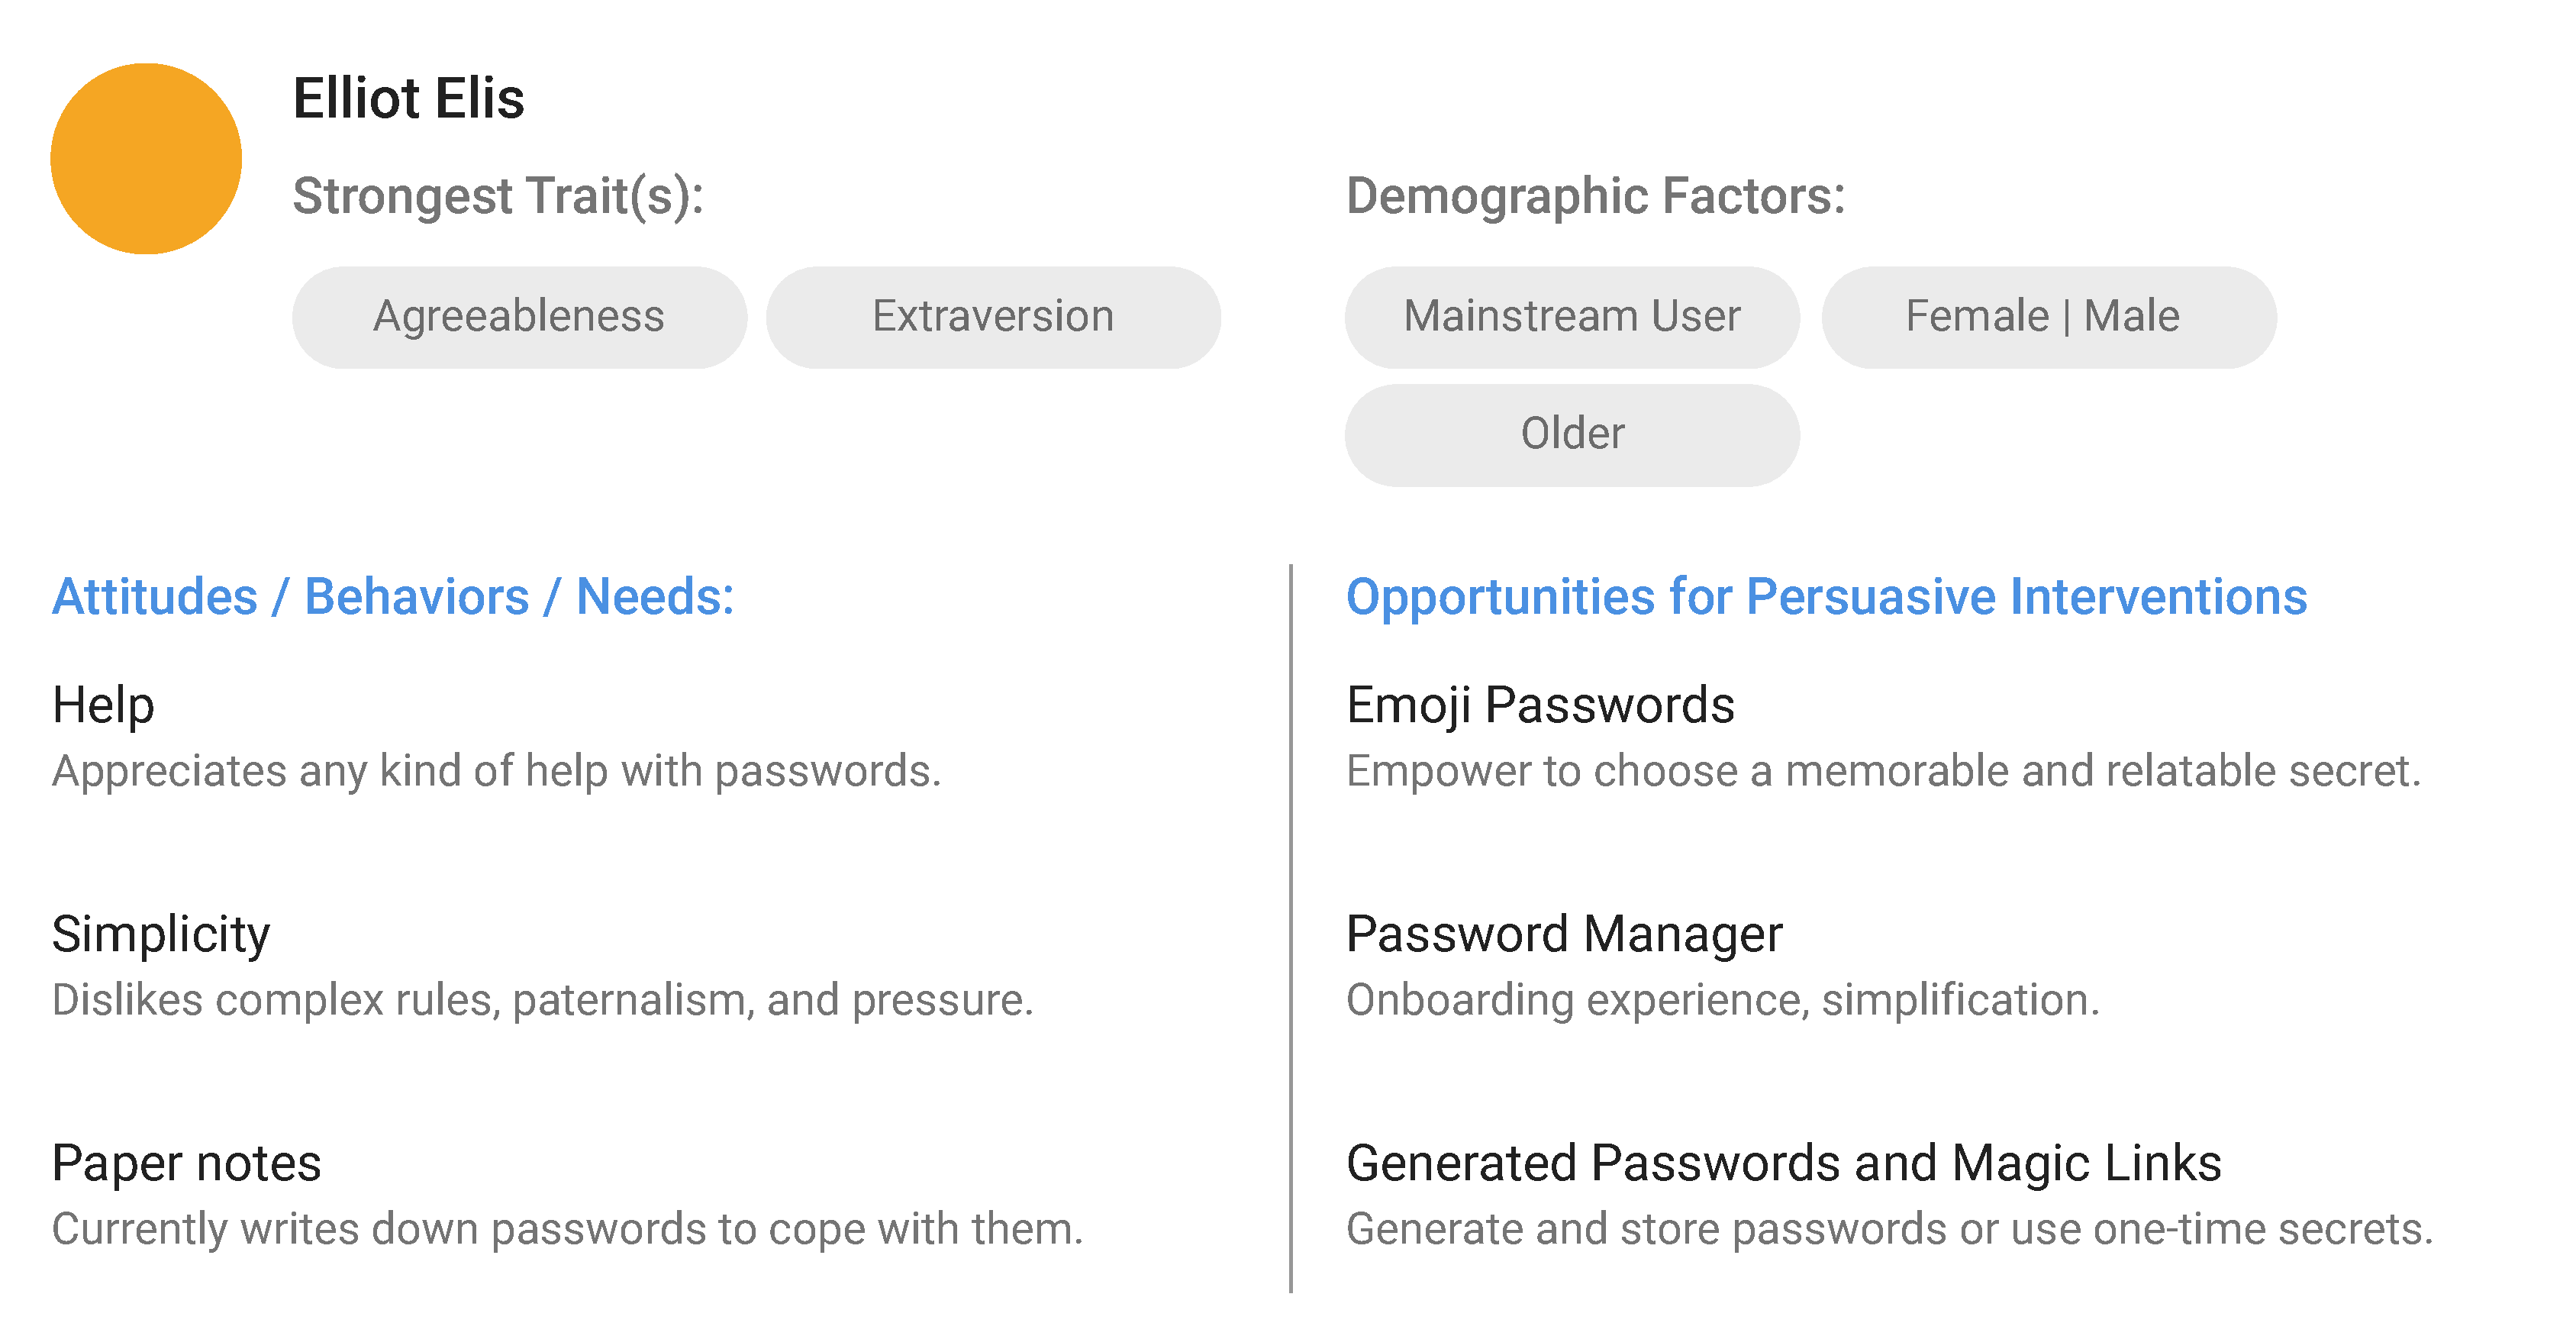
\includegraphics[width=0.7\linewidth]{personality/personas/Agreeable-Persona}}
	\caption{\label{fig:personality:personas} Password Personas. These fictional user profiles can inform design choices for password support strategies. Refining the details needs further research on password personality.}
\end{figure}

\subsection{Designing Feedback and Suggestions}
% strength suggestions
Using our personas, it is possible to address personality facets in real-time feedback during password creation. In the wild, we encounter password meters that estimate the strength of the password and in some cases even provide verbal feedback about what the user can do to improve the password (see  \cite{Carnavalet2014AnalyzingPWStrengthMeters,Wheeler2016zxcvbn}). A simple approach tries to convince the user to pick a stronger password by \textbf{suggesting a new one} or a modified version of the entered password \cite{Forget2008ImprovingPasswordsThroughPersuasion, Seitz2016SuggestionsDecoy, Shay2015SpoonfulOfSugar, Ur2017DataDrivenPWMeter}. 

Coming back to the finding that personality had a notable effect on how participants \textit{compared} two passwords, we suppose that it plays a role for real-time suggestions, too. How a modified version or newly generated password is received likely depends on the user's personality. On mobile devices, the user's password might be visible in clear text while they enter it \cite{Melicher2016UsabilityMobileTextPasswords}. Displaying an alternative password then resembles the comparison task from our study, and they might wonder which one is stronger. Strength feedback facilitates answering this question. It seems to be easier for \textit{conscientious} people to assess the strength of their password, if there is a clear list of requirements than can be ``checked off'', to make it superior to the suggested password (see the persona 3 ``Taylor Tang'' in Figure \ref{fig:personality:personas}). At the same time, users who strongly show the \textit{openness} trait seem to benefit from data-driven background information about the strength estimation algorithm. We conclude that Ur \etal's meter might be especially helpful for the persona 2 (Frankie Fizz). To make it work for persona 1 (Jamey Jones), it needs to be more reassuring than it currently is: The version presented at CHI 2017 constructively criticizes the user's password and suggests alterations. Adding a positive message might make persona 1 more receptive for this kind of suggestions. 

% coping suggestions.
Moreover, we found that demographic factors are useful to segment audiences. We found that older participants in our third study were more likely to appreciate if they do not need to memorize passwords, which was considered in persona 4 (Elliot Elis). They were more likely to use a password manager, paper notes or reusing passwords to reduce cognitive efforts. Thus, there is a great opportunity to suggest a coping strategy instead of a stronger password. For instance, websites or browsers could extend sign-up forms with a prompt to use a password manager. Pointing out the value of not having to memorize the newly created password could speak to older users and drive adoption rates. It is very important that the user journey from sign-up to password-manager set-up is simple enough to meet persona 4's needs. During account creation, interventions can leverage the ``opportune moment'': \textit{Kairos}, one of the persuasion principles presented in Section \ref{sec:rw:persuasive_patterns}, likely possesses a higher nudging power than, e.g. a news article recommending a password manager, because users are experiencing the problem first-hand during account creation. 

%\subsection{Tackling the ``Unknown User'' Problem}

%Results from the first study showed differences in the way participants dealt with password rules. The second study indicated that users the perception of password strength depends on both topology and personality. 

%Identity providers like Facebook or Google still rely on password authentication, and currently implement a ``one-fits-all'' policy. However, once users have used the services for a while, those parties already possess a large amount of user information. Consequently, the identity providers could alter the enforced policy for individual users depending on personality trait characteristics inferred from usage patterns. We propose to dynamically adjust the policy, for example when users reset their password. Users with an IT background could be asked to conform to a complex and long policy, while users showing stronger signs of neuroticism could be nudged towards including an emoji in their password. Such approaches could support the existing mental models of password strength and reduce user frustration with requirements. Ultimately, this can boost usability or user experience of the service. 
%TODO maybe inlcude the above part on emoji passwords / empowerment. 

% How can the segmentation be performed automatically without active user involvement?
% 	difficult questions -- smartphones
\subsection{Assessing Personality Traits in Password Studies}
In our studies, we \textit{explicitly} measured personality through psychometric constructs. This was straightforward, because online studies have become a reliable go-to method to study passwords. However, in many cases, omnibus tests like ANOVAs fail to reveal significant effects, and confounding variables could blur causality. Only few such covariates have been considered beyond demographic information. Our studies highlight that personality is a promising candidate to consider: for instance, average password strength perceptions were distributed normally. However, using general models, the underlying associations became visible and were statistically significant. Thus, psychometrics should not be neglected, so we can boost efficacy of security mitigations for different user segments \cite{Egelman2015AverageUser}. 

Still, extending surveys with long psychometric constructs is probably unrealistic. In our studies we used 50 and 21-item constructs. The latter already showed slightly reduced internal consistency. Thus, to keep studies short, to prevent participant fatigue, and to obtain reliable data, we propose focusing on the \textbf{openness} and \textbf{neuroticism} personality traits. Their associations were most stable in our studies and provided a coherent picture. They can be measured with only a couple of items (between 9 and 20), so the corresponding study part is finished within a few minutes. Nevertheless, the specific choice of the traits should be backed up by confirmatory studies in the future, and may also depend on the research question.

Adding even a few more items to a questionnaire might be impossible due to study constraints like budget or timeliness of data elicitation. There are, however, promising solutions to quickly and inexpensively obtain personality data on all dimensions from a user's past behavior. It is possible to infer personality facets from \textbf{social media data}, e.g. public interactions on Facebook \cite{Youyou2015Personality}. Youyou et al. found that such metrics can even outperform psychometric questionnaires. Stachl et al., as well as De Montjoye \etal found conclusive associations between \textbf{smartphone usage} and personality traits \cite{DeMontjoye2013, Stachl2017PersonalitySmartphones}. We thus suggest requesting permission to read either smartphone or social network data as part of the study. Crowd-workers in a large-scale study by Bentley and Chen, for instance, showed little concern to install software on smartphones for research purposes \cite{Bentley2015Phonebook}. While we would not go so far as to read all contacts, call and message history, we believe a differentially private\footurl{https://en.wikipedia.org/wiki/Differential_privacy}{04.03.2018} approach can replace personality constructs. 

% \todo{This argument is later revisited in the ``ideas'' an/or PST section, so maybe cross-reference it.}
 
\subsection{Statistical Models}
After consultation with statisticians, we opted for the use of generalized additive models (GAMs). Their usefulness hinges on the interpretability of their corresponding regression plots. Traditional indicators like (un-)standardized coefficients are limited in their contribution to gauge marginal associations and must be interpreted with special caution. In the case of logistic regression, standardizing binary variables is not useful, but we reported beta values to describe the slopes in the plots. Especially in study 2, we tried to select the model with the highest goodness of fit as indicated by the adjusted R-square value. We also considered the models' Akaike information criterion (AIC) to move forward. Here, increases and decreases of the AIC matched those of the R-square value. Interestingly, the models achieved better fit than related work on personality in privacy behavior \cite{Egelman2015AverageUser}. Thus, we advocate the use of GAMs in future analyses.  

\section{Conclusion and Future Work}
In three studies with a total of 440 participants, we broadly explored associations between personality traits and password behavior. This effort was one of the first of its kind. We focused on the relationship between the Big-Five model and password policies, strength perceptions, password selection, and coping strategies, while controlling for demographic factors. We found evidence for associations between (a) the usability of password policies and the neuroticism trait; (b) password strength perceptions and openness, respectively conscientiousness; (c) password length and neuroticism; (d) coping strategies and extraversion; and (e) IT-background and more secure behavior. Although the associations were not always particularly strong, they are still useful to inform the design of persuasive interventions and password policies. To that end, a set of four password personas was created to segment user groups by behavioral, attitudinal, and demographic archetypes. 

\subsubsection{Future Work}
Our work was of exploratory nature. Thus, the next step should be a focused study that increases statistical power to confirm or refute the associations. We provided a user segmentation in our personas to derive testable hypotheses. The refined knowledge about personality traits can be used to personalize password feedback and make it more effective. As pointed out by related work, some users overestimate the strength improvement of using digits in passwords \cite{Ur2016PerceptionsPassword}, which we also saw in studies 2 and 3. However, not all participants were equally influenced by digits or different character classes inside passwords. Respecting the psychographics in real-time feedback while carefully enforcing sensible policies could make these messages more effective. Besides, personality traits can inform choice architectures beyond passwords. For example, the Choose-Your-Own-Authentication approach \cite{Forget2015CYOA} can benefit from improved default settings depending on personality trait characteristics. The collection and aggregation of the necessary information could be done implicitly on mobile phones or social networks \cite{DeMontjoye2013, Stachl2017PersonalitySmartphones, Youyou2015Personality}. We see this a promising opportunity to improve the user experience of authentication mechanisms, because off-the-shelf technology can already achieve this goal. Finally, in light of some participants being more positive towards including emoji in their passwords opens new possibilities for password authentication. Emoji usage itself has been shown to be associated with personality \cite{Marengo2017EmojiPersonality}, which is supported by our research. Thus, it is important to investigate how personality traits might be exploited to model password strength of emoji-passwords. 

%TODO constellations like myers-briggs personality

\noindent
\fbox{
	\label{sec:personality:take-aways}
	\hspace{1cm}
	\parbox[c][15cm]{0.7\linewidth}{
		\section*{Take Aways}
		\begin{itemize}[leftmargin=*]
			\item Personality was weakly associated with all the measured dimensions: strength perception, policy preference / usability, password selection and coping strategies. Most notably openness, conscientiousness and neuroticism showed the most conclusive associations.
			\item The models for the perception of passphrases achieved the highest fit, suggesting a predictable association between personality and strength perception for this type of password. Comparing two passwords was associated with the conscientiousness traits. Mixed models that use both password features and personality trait scores as covariates were the most feasible approach to improve model fit.
			\item We can use ``Password personas'' to inform design decisions of persuasive interventions in the future. For instance, older users might be the best target group for password support tools, because age was a good predictor of their usage. Suggesting good tools during account creation might lead to higher adoption. Nudges designed for neuroticism should make emotional state more salient and positively reinforce the benefits of \underline{long} passwords. 
		\end{itemize}
	}
	\hspace{1cm}
}

